% This is a template for Ph.D. dissertations in the UCI format.
% Modified by Matt Bovyn to serve as an advancement document
% (not for publication)
% 
% All fonts, including those for sub- and superscripts, must be 10
% points or larger.  Recommended sizes are 14-point for chapter
% headings, 12-point for the main body of text and figure/table
% titles, and 10-point for footnotes, sub- and super-scripts, and text
% in figures and tables.
%
% Notes: Add short title to figures, sections, via square brackets,
% e.g. \section[short]{long}.
%
\documentclass[12pt,fleqn]{ucithesis}

% A few common packages
\usepackage{amsmath}
\usepackage{amsthm}
\usepackage{array}
\usepackage{graphicx}
\usepackage{natbib}
\usepackage{relsize}
\usepackage{floatrow}
\usepackage{enumitem} %for indenting items in description environment

% Some other useful packages
\usepackage{caption}
\usepackage{subcaption}  % \begin{subfigure}...\end{subfigure} within figure
\usepackage{multirow}
\usepackage{tabularx}
\usepackage{siunitx}
\sisetup{detect-weight=true, detect-family=true}
\usepackage{physics} %for \vqty, \dd, \dv
\usepackage{changes}
\definechangesauthor[name={Matt Bovyn},color=blue]{MB}

%for nicer Tau
\usepackage{ upgreek }
\renewcommand{\tau}{{\,\uptau}}

% plainpages=false fixes the "duplicate ignored" error with page counters
% Set pdfborder to 0 0 0 to disable colored borders around PDF hyperlinks
\usepackage[plainpages=false,pdfborder={0 0 0}]{hyperref}

% Uncomment the following two lines to use the algorithm package,
% which provides an algorithm environment similar to figure and table
% ("\begin{algorithm}...\end{algorithm}"). A list of algorithms will
% automatically be added in the preliminary pages. Note that you
% probably want a package for the actual code to go with this (e.g.,
% algorithmic).
%\usepackage{algorithm}
%\renewcommand{\listalgorithmname}{\protect\centering\protect\Large LIST OF ALGORITHMS}

% Uncomment the following line to enable Unicode support. This will allow you
% to enter non-ASCII characters (such as accented characters) directly without
% having to use LaTeX's awkward escape syntax (e.g., \'{e})
% NOTE: You may have to install the ucs.sty package for this to work. See:
% http://www.unruh.de/DniQ/latex/unicode/
%\usepackage[utf8x]{inputenc}
%\usepackage[T1]{fontenc}

% Uncomment the following to avoid "widowing", where page breaks cause
% single lines of paragraphs to float onto the next page (this is not
% a UCI requirement but more of an aesthetic choice).
%\widowpenalty=10000
%\clubpenalty=10000

% Modify or extend these at will.
\newtheorem{theorem}{\textsc{Theorem}}[chapter]
\newtheorem{definition}{\textsc{Definition}}[chapter]
\newtheorem{example}{\textsc{Example}}[chapter]

% Macros for title, author, abstract, etc.
\thesistitle{Cargo Navigation Across 3D Microtubule Intersections}

\degreename{Master of Science}

% Use the wording given in the official list of degrees awarded by UCI:
% http://www.rgs.uci.edu/grad/academic/degrees_offered.htm
\degreefield{Physics}

% Your name as it appears on official UCI records.
\authorname{Matthew Jacob Bovyn}

% Use the full name of each committee member.
\committeechair{Professor Jun Allard}
\othercommitteemembers
{
  Professor Steve Gross, Co-Advisor\\
  Professor Albert Siryaporn
}

\degreeyear{2017}

\copyrightdeclaration
{
  {\copyright} {\Degreeyear} \Authorname
}

% If you have previously published parts of your manuscript, you must list the
% copyright holders; see Section 3.2 of the UCI Thesis and Dissertation Manual.
% Otherwise, this section may be omitted.
% \prepublishedcopyrightdeclaration
% {
% 	Chapter 4 {\copyright} 2003 Springer-Verlag \\
% 	Portion of Chapter 5 {\copyright} 1999 John Wiley \& Sons, Inc. \\
% 	All other materials {\copyright} {\Degreeyear} \Authorname
% }

% The dedication page is optional.
%\dedications
%{
%  (Optional dedication page)
%  
%  To ...
%}

\acknowledgments
{
Foremost, I'd like to thank my advisors Jun Allard and Steve Gross for their constant support. I would also like to thank my lab mates in the Allard Lab (Lara Clemens, Abdon Iniguez, Kathryn Manakova, and Derek Bryant) and in the Gross Lab (Babu Reddy and Dail Chapman) for productive conversations and general help of all kinds. I would also like to thank the members of the UCI Center for Biological Systems for productive and enlightening conversations, as well as the training I needed to take on this project.

I was supported by NIH T32 EB009418-07 to Arthur Lander and Qing Nie, as well as NIH R01 GM123068 to Jun Allard and Steve Gross.
  
  You also need to acknowledge any publishers of your previous
  work who have given you permission to incorporate that work
  into your dissertation. See Section 3.2 of the UCI Thesis and
  Dissertation Manual.)
}


% Some custom commands for your list of publications and software.
\newcommand{\mypubentry}[3]{
  \begin{tabular*}{1\textwidth}{@{\extracolsep{\fill}}p{4.5in}r}
    \textbf{#1} & \textbf{#2} \\ 
    \multicolumn{2}{@{\extracolsep{\fill}}p{.95\textwidth}}{#3}\vspace{6pt} \\
  \end{tabular*}
}
\newcommand{\mysoftentry}[3]{
  \begin{tabular*}{1\textwidth}{@{\extracolsep{\fill}}lr}
    \textbf{#1} & \url{#2} \\
    \multicolumn{2}{@{\extracolsep{\fill}}p{.95\textwidth}}
    {\emph{#3}}\vspace{-6pt} \\
  \end{tabular*}
}

% Include, at minimum, a listing of your degrees and educational
% achievements with dates and the school where the degrees were
% earned. This should include the degree currently being
% attained. Other than that it's mostly up to you what to include here
% and how to format it, below is just an example.
\curriculumvitae
{

\textbf{EDUCATION}
  
  \begin{tabular*}{1\textwidth}{@{\extracolsep{\fill}}lr}
    \textbf{Doctor of Philosophy in Computer Science} & \textbf{2012} \\
    \vspace{6pt}
    University name & \emph{City, State} \\
    \textbf{Bachelor of Science in Computational Sciences} & \textbf{2007} \\
    \vspace{6pt}
    Another university name & \emph{City, State} \\
  \end{tabular*}

\vspace{12pt}
\textbf{RESEARCH EXPERIENCE}

  \begin{tabular*}{1\textwidth}{@{\extracolsep{\fill}}lr}
    \textbf{Graduate Research Assistant} & \textbf{2007--2012} \\
    \vspace{6pt}
    University of California, Irvine & \emph{Irvine, California} \\
  \end{tabular*}

\vspace{12pt}
\textbf{TEACHING EXPERIENCE}

  \begin{tabular*}{1\textwidth}{@{\extracolsep{\fill}}lr}
    \textbf{Teaching Assistant} & \textbf{2009--2010} \\
    \vspace{6pt}
    University name & \emph{City, State} \\
  \end{tabular*}

\pagebreak

\textbf{REFEREED JOURNAL PUBLICATIONS}

  \mypubentry{Ground-breaking article}{2012}{Journal name}

\vspace{12pt}
\textbf{REFEREED CONFERENCE PUBLICATIONS}

  \mypubentry{Awesome paper}{Jun 2011}{Conference name}
  \mypubentry{Another awesome paper}{Aug 2012}{Conference name}

\vspace{12pt}
\textbf{SOFTWARE}

  \mysoftentry{Magical tool}{http://your.url.here/}
  {C++ algorithm that solves TSP in polynomial time.}

}

% The abstract should not be over 350 words, although that's
% supposedly somewhat of a soft constraint.
\thesisabstract
{
  Eukaryotic cells maintain a high level of internal organization and change it dynamically to respond to their environment. The localization of organelles such as mitochondria and lipid droplets is often determined by their transport along the microtubule cytoskeleton by molecular motors in the kinesin superfamily and cytoplasmic dynein. The single molecule function of these motors has been intensely studied, but it remains unclear how the motile properties of these molecules are harnessed by the cell to localize cargos to the correct place. The work in this document explores how the properties of the motors, the cellular environment, and the cargos themselves conspire direct intracellular traffic. First, we explore how the organization of a basic element of the cellular environment --- the microtubule cytoskeleton --- can determine cargo routing. In a second project, I propose to investigate how the manner in which motors are attached to the cargo can influence transport. In a third project, I propose a combination of experimental and computational studies to examine the relationship between the binding rate of individual motor proteins to microtubules and binding rates of the cargos they are attached to. Furthermore, I propose to investigate how modulation of this relationship may allow the cell to regulate transport.
  
   Active transport of intracellular cargos along microtubules is essential for organization and function of eukaryotic cells. The properties of the molecular motor proteins that power this transport have been intensely studied on the single molecule level, but it remains unclear how these motors function in groups and how the cell controls the function of the motors to deliver cargos to the correct place at the correct time. Furthermore, the cell must direct the transport of a variety of cargos with different destinations along the same network of microtubule ``roadways'', using the same set of molecular motors to power their transport. The projects presented here address mechanisms by which the cell might achieve this multiplexed control.

The projects investigate cargo transport through mathematical models and through experiments, both in vitro and in cells. The mathematical models are derived by using force balance to find the equations of motion for the cargo, modeled as a spherical rigid body. A Brownian force term is included, making the equations stochastic. To solve these equations, along with implementing motor stepping, binding and unbinding, we've written a hybrid Euler-Maryuama-Gillespie simulation. The experiments make use of differential interference contrast microscopy to visualize cells and organelles, particularly lipid droplets. Optical tweezers are used to measure forces on cargos created by molecular motors both in vitro and in cells.
  
  In collaboration with the Vershinin Lab at University of Utah, we investigate how cargos navigate microtubule intersections in 3D. While cargo transport is often studied only along a single microtubule, the microtubule network is usually a dense mesh, with microtubules frequently crossing each other close enough together for cargos to encounter both microtubules simultaneously. When cargos encounter such an intersection, do they switch to the intersecting microtubule or pass it by? The Vershinin Lab conducted a series of in vitro experiments with kinesin motors attached to glass bead cargos and found that the probability for the cargo to switch tracks depends strongly on the geometry of the intersection. We constructed a simulation to investigate how the properties of the molecular motors and cargo lead to the switching probabilities observed. We report that well known properties of the molecular motors lead to switching probabilities close to those observed in experiment. Furthermore, we report that observed switching probabilities stem from unexpected effects, such as cargo diffusion being constrained by motors bound to the microtubule. \textbf{Our results predict high switching rates for intersections in which microtubules are spaced less than one quarter of a cargo diameter apart, suggesting the cell could regulate switching by modulating microtubule spacing.} In this work, theory allows insight into mechanisms which would otherwise be unobservable (either because of experimental limitations, like finding the number of motors engaged, or because they are in general not directly observable, like force states). This insight allows us to predict what features of the experimental data are likely to generalize to other cargos and in vivo situations, and which are not. This work is currently in revision.
}


%%% Local Variables: ***
%%% mode: latex ***
%%% TeX-master: "thesis.tex" ***
%%% End: ***


% Add PDF document info fields
\hypersetup{
	pdftitle={\Thesistitle},
	pdfauthor={\Authorname},
	pdfsubject={\Degreefield},
	colorlinks=true,
	urlcolor=blue,
	citecolor=black,
	linkcolor=black,
}

% Uncomment the following to have numbered subsubsections (by default
% numbering goes only to subsections).
%\setcounter{secnumdepth}{4}


% Set this to only select a subset of the includes directives below.
% Very handy to speed up compilation if you're working on a certain
% part of your thesis. It conserves page numbers, references, etc.
% even for non-included files.
%\includeonly{appendix2/appendix2}

\begin{document}

% Preliminary pages are always loaded (TOC, CV, etc.)
\preliminarypages

% Include the different components of your thesis, in separate files.
% Using \include allows you to set \includeonly above.
\chapter{Introduction}

Life on earth is mindblowingly diverse. For anything you might try to pin down as the defining feature --- be it DNA, metabolism, reproduction, or anything else you can dream of, counterexamples and edge cases spring up to defeat you. It is instructive to look instead not at individual elements, but at design principles: what are the common ways evolution has wrangled various arrangements of carbon, nitrogen, oxygen and other trace elements to build up bacteria, elephants, and jelly fish? (Not to mention the human that wrote the words on this page, and the one reading them.) One fundamental motif is the barrier; all life on earth uses barriers to contain the chemical reactions which give rise to the properties we associate with being alive: movement, metabolism, reproduction, and so on.

While bacteria have only a single major barrier which functions to separate their carefully controlled interior environment from the outside world, eukaryotic cells have in addition developed a multitude of internal barriers. To construct these internal barriers, eukaryotic cells mostly use lipid bilayers. The organelles encapsulated by these internal barriers allow eukaryotic cells to maintain a variety of vastly different chemical environments, which together can be used to accomplish complex tasks not achievable in any one environment alone. 

For this strategy to succeed in keeping the cell functioning, different enclosed environments need to communicate with one another. While communication is possible at a distance, it is often more effective --- and sometimes necessary --- for organelles to make physical contact with each other to transfer molecules or pass along signals. Controlling contact between organelles --- and more generally controlling cell spatial organization --- requires that organelles move around relative to each other. While thermal energy causes significant motion even on the scale of an organelle, the relatively weak and undirected motion is not sufficient for delivering cargos in a reasonable time. 

To this end, eukaryotic cells have built up a complex transport system to control the organization of their organelles in space and time. To transport organelles, eukaryotic cells have evolved to use molecular motors, which transform the cell's chemical energy currency, ATP, into mechanical work. These motors move along filamentous tracks: the molecular motors kinesin and dynein move along the large, rigid microtubules, while myosin motors move along the thinner, more floppy actin filaments.

The general question which naturally arises from the ideas so far established is this: how does the cell control the transport of various cargos from one place to another? There are many types of cargos, each of which with different functions which may necessitate them to be localized differently from each other at different times. How is intracellular traffic directed? This is the question we will concern ourselves with.

\chapter{Background} \label{ch:background}

The advent of video microscopy brought the dynamic nature of the organelle environment into focus in the early 1980s \cite{Allen1981,Inoue1981}. Soon after, Ron Vale and colleagues discovered the identity of one of the proteins responsible for the observed transport, kinesin \cite{Vale1985}. In the more than 30 years since this discovery, we have learned a great deal about each of the components of the transport system from a combination of careful in vivo and in vitro experimental work, as well as enlightening modeling efforts.

\section{Microtubules}

Eukaryotic cells possess a microtubule (MT) network, composed of hundreds of individual MT filaments. Recently, super-resolution microscopy has allowed imaging and mapping of the entire MT network with single MT resolution \cite{Zhang2016}, as shown in figure \ref{fig:MTcytoskeleton}. Individual MTs are dynamic, assembling and disassembling stochastically \cite{Howard2003}. This allows the MT network to be reorganized as cells move and change shape, as well as in response to external cues \cite{Herms2015,Zhu2015,Zhang2016}. 

\begin{figure}
\centering
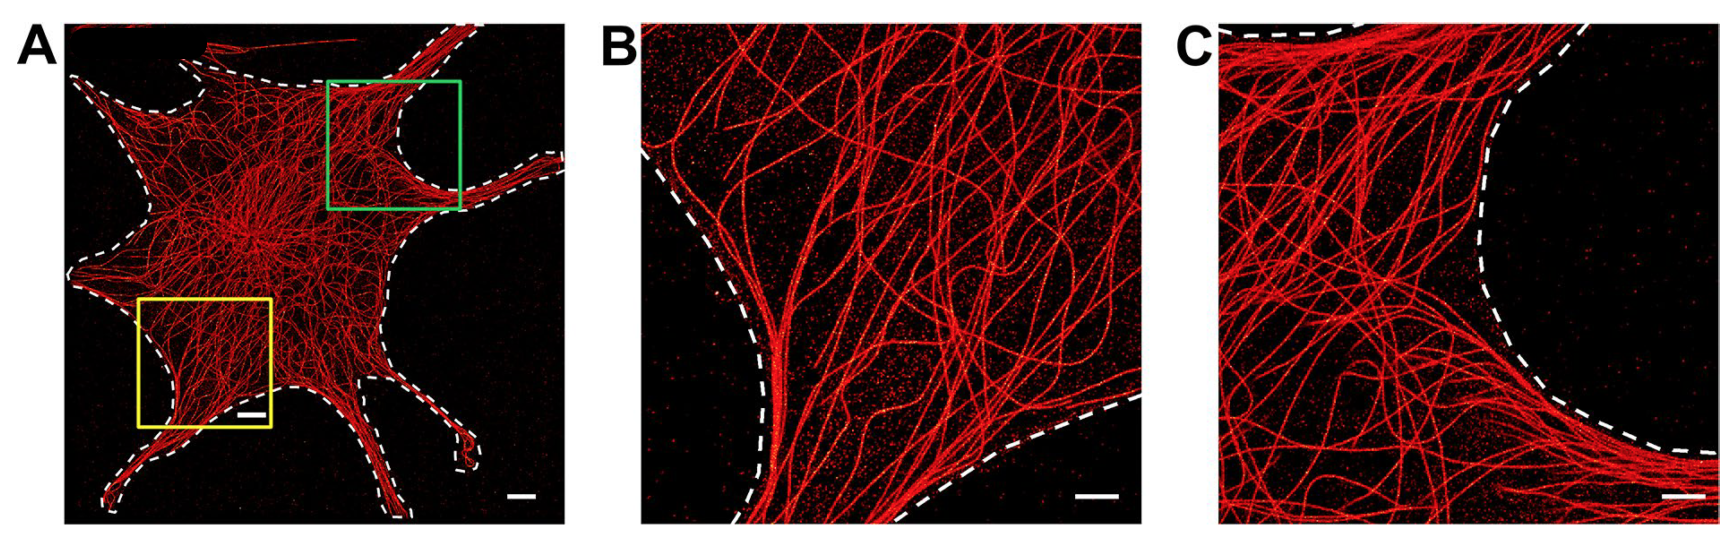
\includegraphics[scale=.5]{background/MTcytoskeleton}
\caption[Super-resolution image of a MT network]{An example of a super-resolution image of an entire MT network of a cell (A), adapted from \cite{Zhang2016}. Single MTs are identifiable from fluorescence labelling in red. Region in yellow box magnified in (B), region in green box magnified in (C). Scale bars are \SI{5}{\micro\meter} in panel A and \SI{2}{\micro\meter} in panels B and C.}
\label{fig:MTcytoskeleton}
\end{figure}

The MT network serves many functions in the cell. Most importantly for the work in this document, MTs serve as the ``roads'' along which cargos are transported. In addition to this role, MTs are a component of the of the cytoskeleton, which gives cells shape and structure. Furthermore, MTs bear the forces exerted to divide chromosomes between the daughter cells in cell division. 

The structure of MTs allow them to perform these functions. MTs are tubular, consisting of a number of linear protofilaments assembled into a ring \cite{Grimstone1966} as shown in figure \ref{fig:MTstructure}. MTs commonly have 13 or 14 protofilaments \cite{Pierson1978}, but that number can vary from fewer than 9 to more than 15 depending on organism and cell type \cite{Davis1983}. Each protofilament is a repeating polymer of dimers of $\alpha$ and $\beta$ tubulin subunits. This repeating structure makes it possible for kinesin and dynein to move processivley along the MT outer surface. MT structures can have defects, and it has been shown these defects can influence transport \cite{Liang2016}.

\begin{figure}
\floatbox[{\capbeside\thisfloatsetup{capbesideposition={right,top}}}]{figure}[\FBwidth]
{\caption[Microtubule Structure]{The structure of a microtubule is shown, demonstrating the tubular structure composed of linear protofilaments made up of repeating dimers of $\alpha$ and $\beta$ subunits. Illustration \href{https://en.wikipedia.org/wiki/Microtubule\#/media/File:Microtubule_structure.png}{``Structure of a microtubule''} by \href{https://commons.wikimedia.org/wiki/User:Splette}{Thomas Splettstoesser} is licensed under \href{https://creativecommons.org/licenses/by-sa/4.0/}{CC BY-SA 4.0.}}
\label{fig:MTstructure}}
{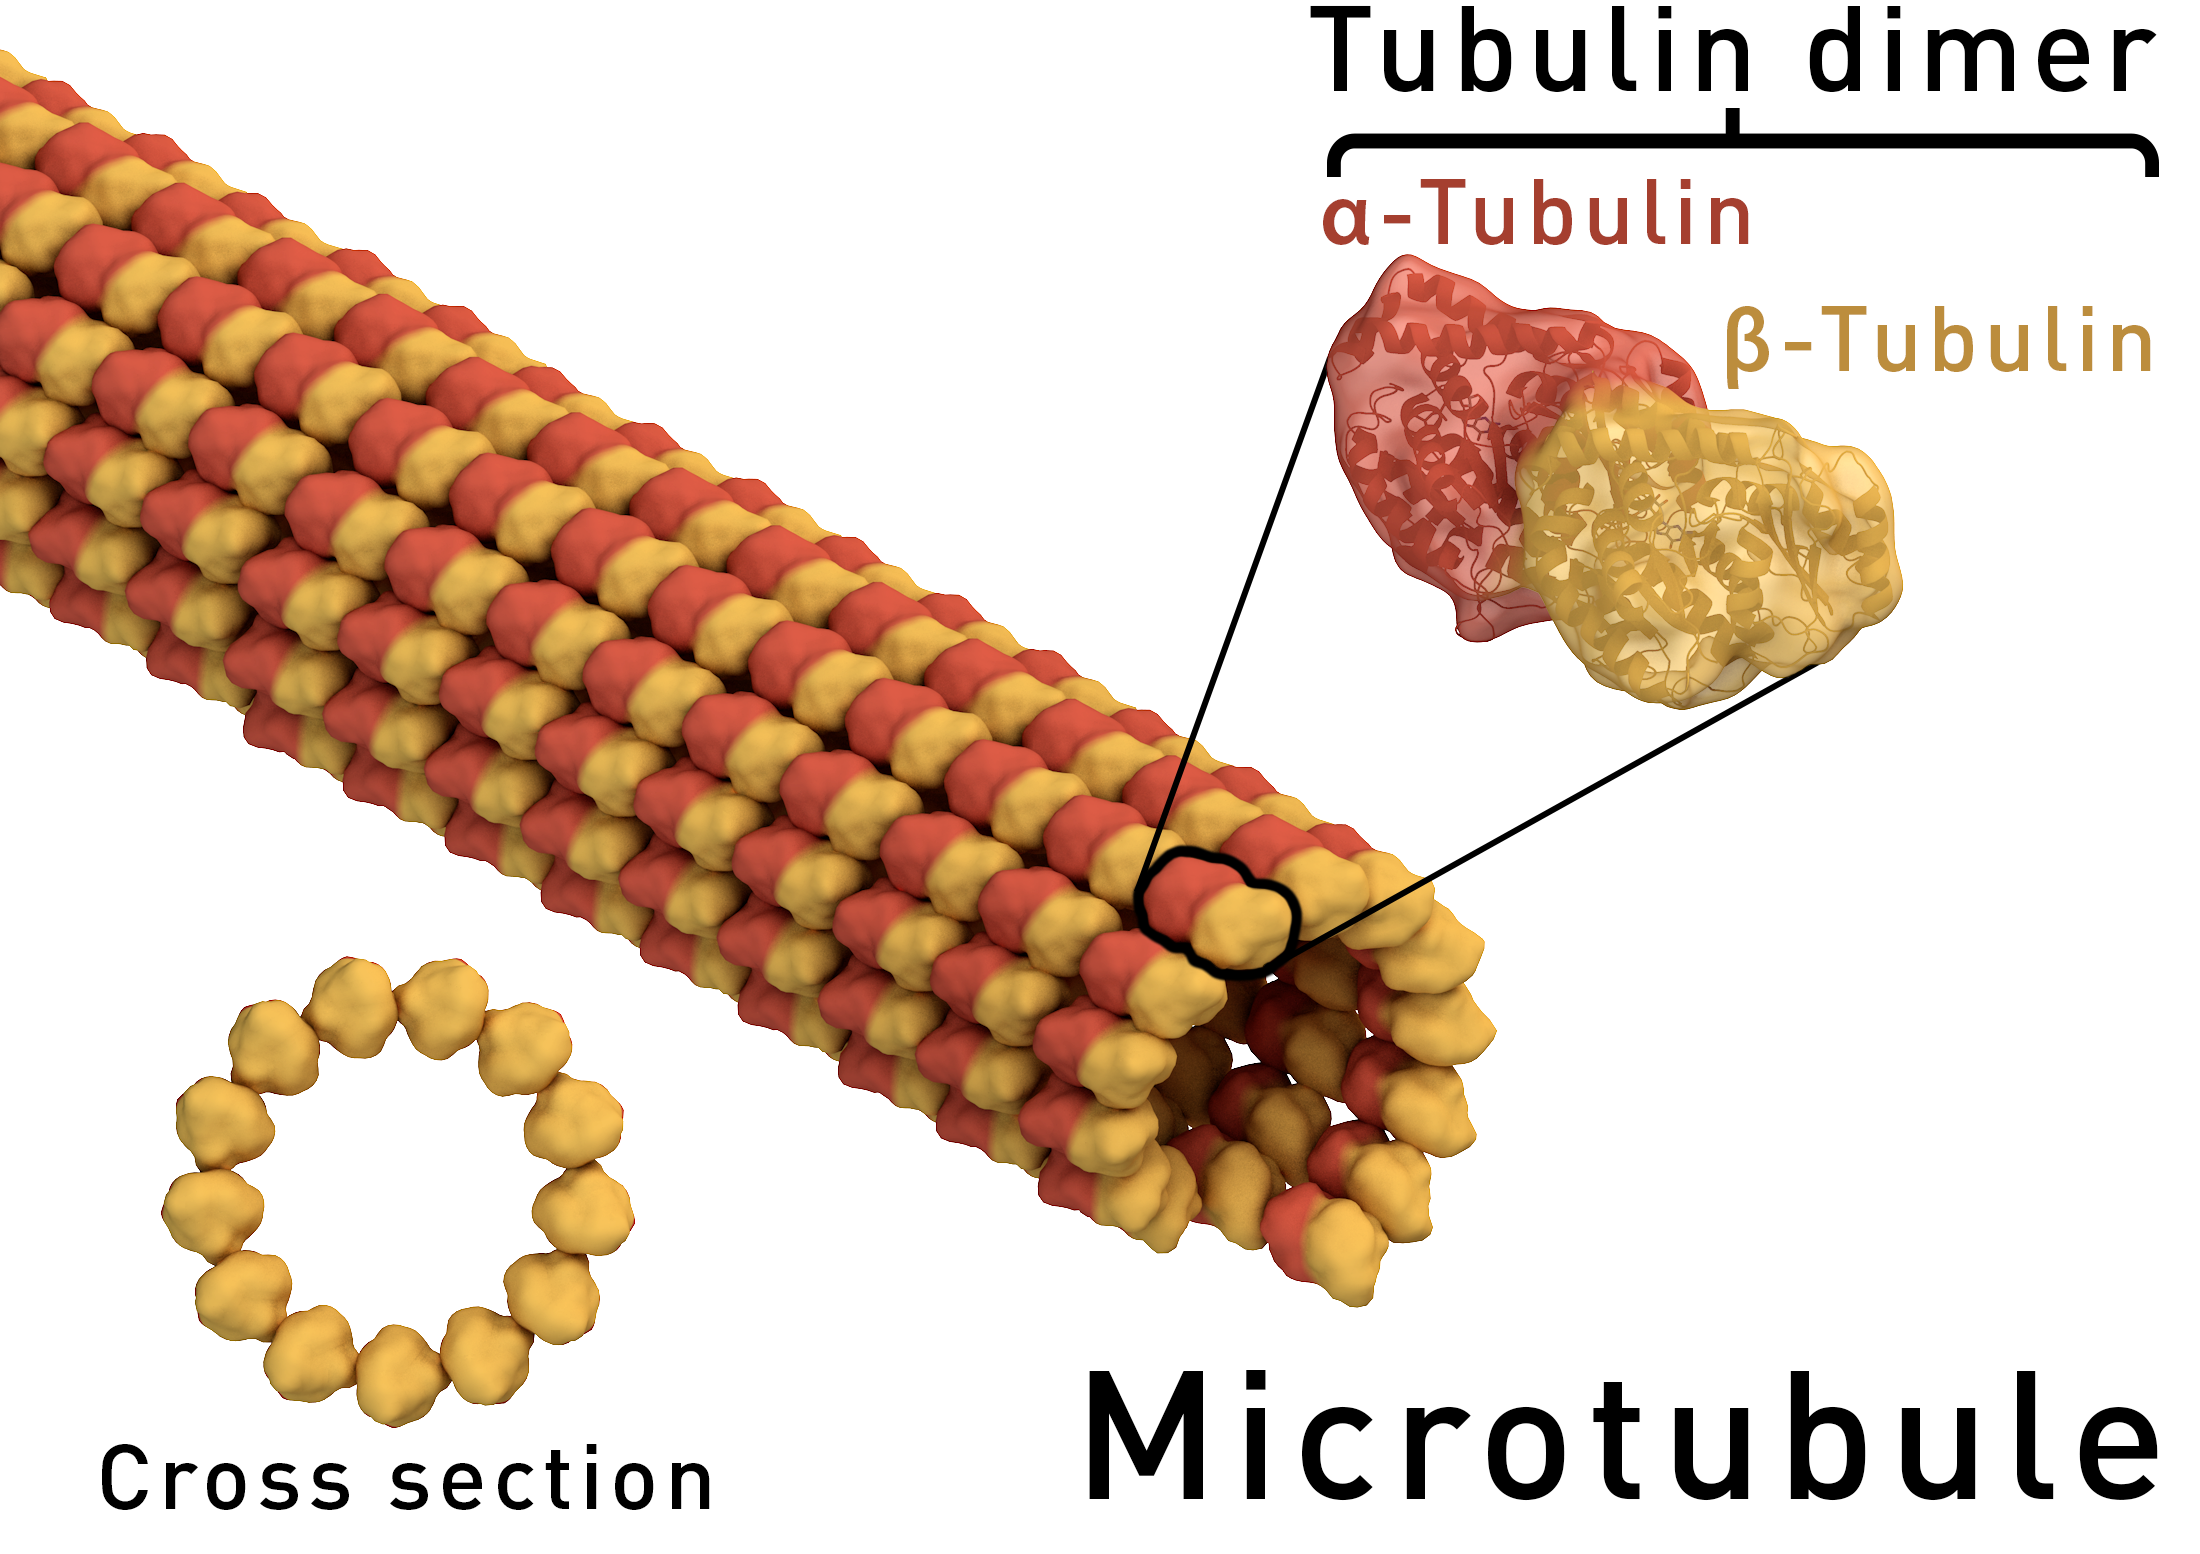
\includegraphics[scale=.1]{background/Microtubule_structure}}
\end{figure}

The tubular structure makes MTs rigid, with persistence lengths near \SI{1}{\milli\meter}, many times the size of an entire cell. Rigidity can vary with MT length and repeated bending \cite{Schaedel2015}.

\section{Molecular Motors}

Molecular motors are a class of enzymes (specifically ATPases), which convert the chemical energy of ATP into mechanical work. There are three classes of molecular motors involved in cargo transport: kinesin superfamiliy motors and cytoplasmic dynein which walk along microtubules, and myosin superfamily motors which walk along actin. Here we'll focus on kinesin.

\subsection{Kinesin} \label{sec:kinesin}

The defining feature of a kinesin is the kinesin motor domain, which binds to MTs and is responsible for ATP hydrolysis \cite{Verhey2011}. Hundreds of genes which include the kinesin motor domain have been identified across a variety of different organisms; together these genes make up the kinesin superfamily. This superfamily has been divided into 14 families based on function and sequence similarity \cite{Lawrence2004}. In mice, there are 45 individual kinesins which perform a variety of tasks in the cell, from transporting cargo to MT depolymerization \cite{Hirokawa2009}. The motors which have established roles in transport are the members of the kinesin-1 (KIF5), kinesin-2 (KIF3) and kinesin-3 (KIF1) families \cite{Verhey2011}. Kinesin-1 is the most well studied family, also called conventional kinesin. It is a heterotetramer of a kinesin heavy chain homodimer and two kinesin light chain subunits, as shown in figure \ref{fig:kinesin_types}. Kinesin-2 can exist either as a homodimer or heterodimer of different motor domain containing subunits, with each form associated with different motility properties. However, the motility mechanism of kinesin-2 is similar to kinesin-1 \cite{Andreasson2015b}. Kinesin-2 motors also tend to switch protofilaments while walking, resulting in a spiral path around the MT \cite{Brunnbauer2012}, where kinesin-1 motors walk a straight line \cite{Ray1993}. Kinesin-3 motors exhibit limited motility as a monomer, but likely work as dimers in vivo, similar to kinesin-1 and kinesin-2 motors \cite{Siddiqui2017}. We will focus on kinesin-1 for the rest of this section and will refer to it simply as kinesin.

\begin{figure}
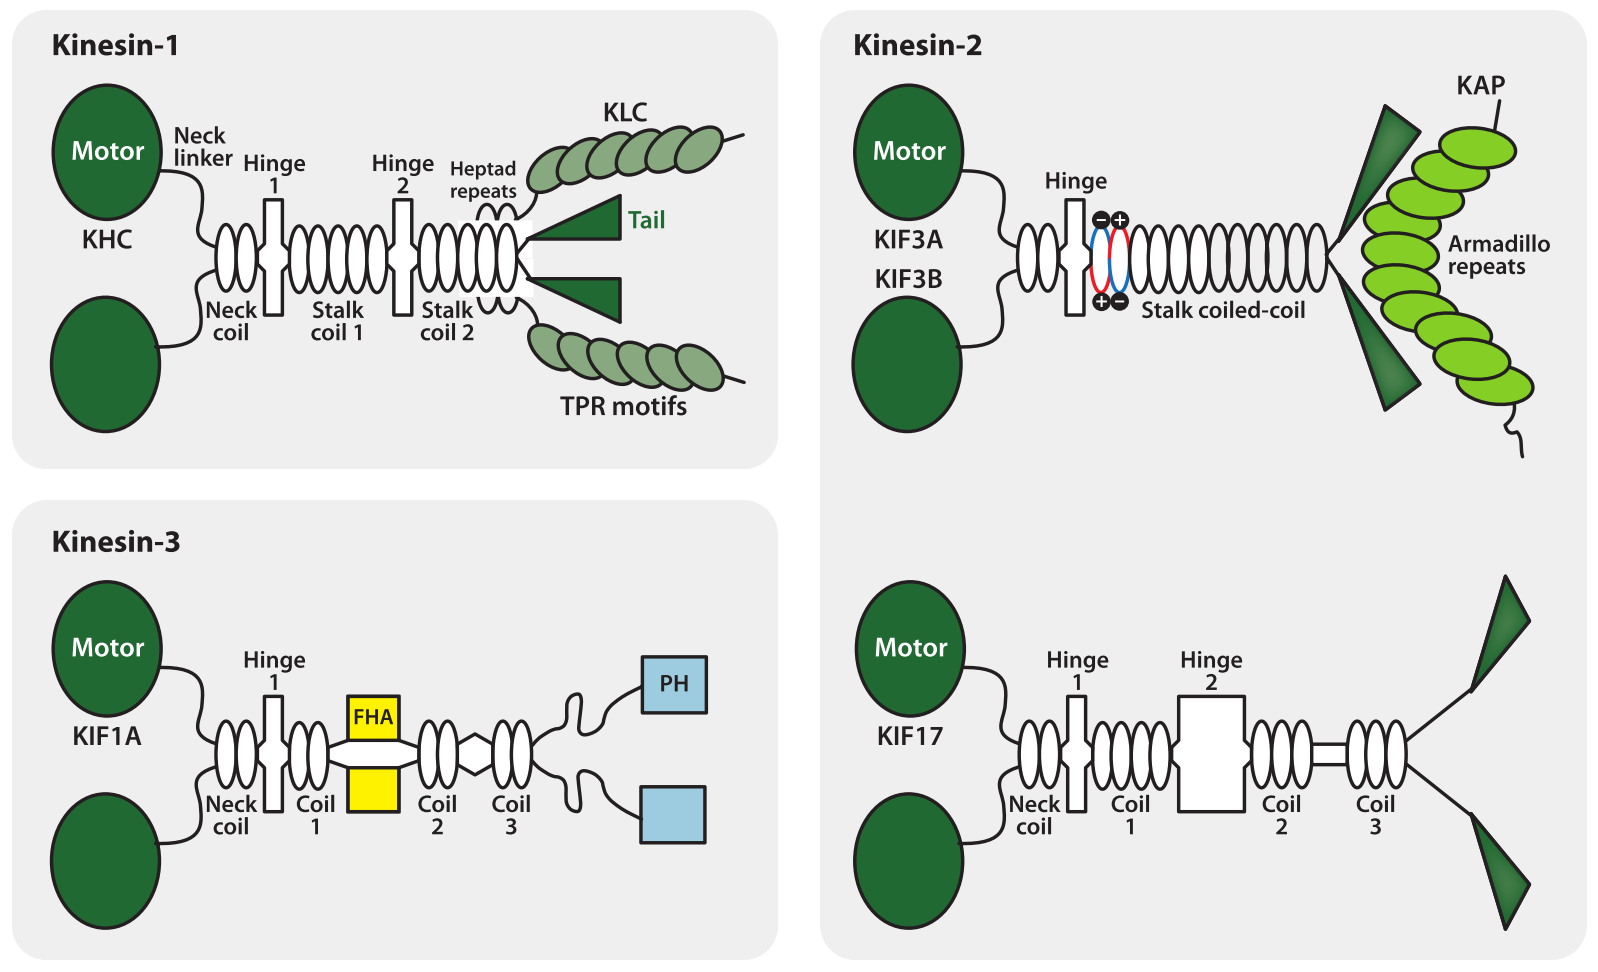
\includegraphics[width=\textwidth]{background/kinesin_types}
\caption[Composition of transport kinesins]{Subunit composition of transport kinesins. Kinesin-1 or conventional kinesin is the most well studied motor family. Kinesin-2 and kinesin-3 are less studied, but also known to transport cargos in cells. Kinesin motor domins are the defining feature of the kinesin superfamily and are shown as green ovals. Kinesin motors domains bind to the MT, which the other end of the motors bind cargos or linkers. Abbreviations: FHA, forkhead associated; KAP, kinesin-associated protein; KHC, kinesin heavy chain; KIF, kinesin family; KLC, kinesin light chain; PH, pleckstrin homology; TPR, tetratricopeptide repeat. Figure from \cite{Verhey2011}.}
\label{fig:kinesin_types}
\end{figure}

Kinesin motors step processively along MT tracks in a hand-over-hand fashion, with each motor domain taking \SI{16}{\nano\meter} steps \cite{Yildiz2004} that move the center of mass of the motor forward by \SI{8}{\nano\meter} \cite{Svoboda1993}. When unloaded, kinesin steps quickly, moving about \SI{1}{\micro\meter\per\second}. Times between steps are exponentially distributed \cite{Carter2005}. Velocity reduces under increasing resistive load until stall, which occurs at $\approx$ \SI{6}{\pico\newton}. The nature of this decrease has been found to be superlinear in some studies \cite{Kunwar2010,Visscher1999,Fallesen2011,Rai2013}, while others find more linear behavior \cite{Svoboda1994,Andreasson2015a}.

Kinesin unbinds from the microtubule at a rate that also depends on the load experienced by the motor. Several reports agree that unbinding rate increases with load exponentially up to the stall force, but disagree about behavior above stall. One study claims unbinding rate increases only slowly above stall \cite{Kunwar2011}, while another claims unbinding rate continues to increase exponentially \cite{Andreasson2015a}. The unbinding rate has been found to depend on the directionality of the load applied. Hindering loads result in the aforementioned behavior, while assisting loads result in an increased unbinding rate \cite{Milic2014,Andreasson2015a}. Sideways loads result in slightly asymmetrical unbinding behavior \cite{Block2003}.

It has been found that the kinesin stalk is stiff in tension \cite{Kojima1997} and also resists compression to a lesser degree \cite{Jeney2004}. It has little resistance to torsion \cite{Hunt1993,Gutierrez-Medina2009}.

\section{Cargos}

A wide variety of organelle cargos such as lipid droplets, mitochondria, melanosomes, peroxisomes, pigment granules, endosomes, secretory vesicles, RNA granules, and virions are transported bi-directionally by molecular motors \cite{Hancock2014,Gross2004}. Long distance cargo transport is also particularly important in neurons. Cargos such as dense core vesicles carrying neuropeptide and synaptic vesicles carrying neurotransmitter must be transported down the length of axons, often millimeters to centimeters long, and delivered at presynapses \cite{Maeder2014}. These observations lead to a picture of cargo transport where bidirectional motion is controlled to correctly localize cargos, as shown in figure \ref{fig:cargo_delivery}.

\begin{figure}
\centering
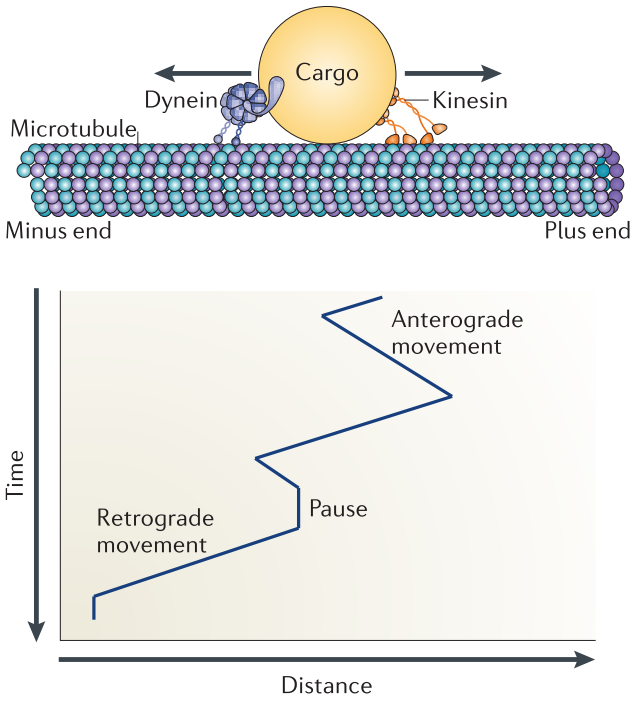
\includegraphics[width=.45 \textwidth]{background/bidirectional_motion}
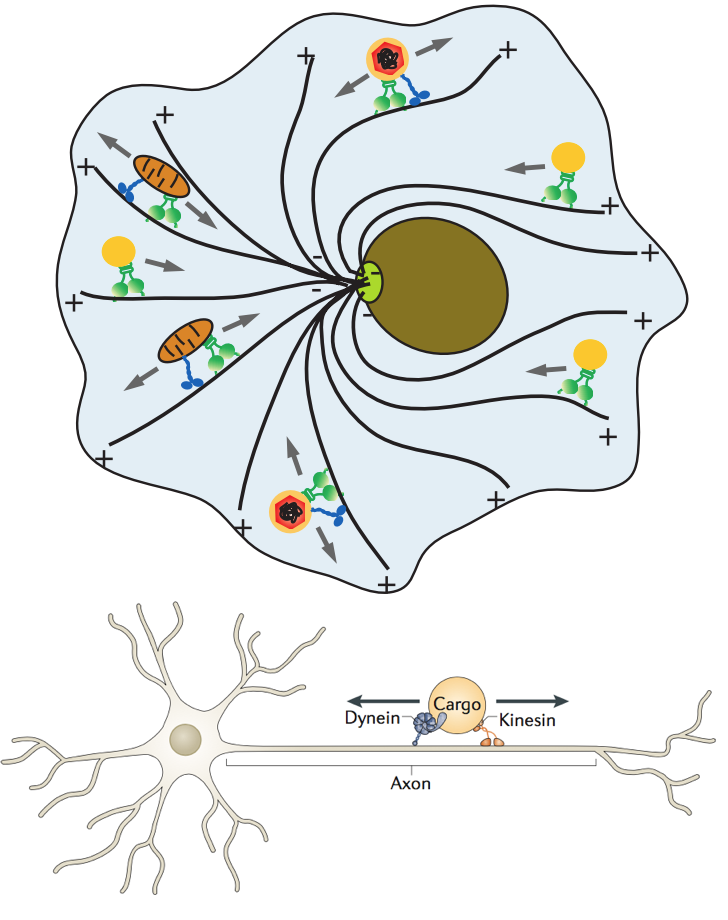
\includegraphics[width=.45 \textwidth]{background/cargo_delivery}
\caption[Bidirectional motion and cargo delivery]{A variety of cargos have been shown to move bidirectionally on MTs in cells, as shown on the left. By biasing this bidirectional motion, the cell may be able to deliver cargos to specific locations in neurons and other cell types, as shown on the right. Figures on left and bottom right from \cite{Hancock2014}. Figure on top right from \cite{Gross2004}.}
\label{fig:cargo_delivery}
\end{figure}

\section{Previous models of cargo transport}

An early model of multiple motor cargo transport posed the problem as a Markov chain, with state transitions representing binding and unbinding of the motors \cite{Klumpp2005}. It was shown this model was able to reproduce a variety of the behaviors observed in vivo \cite{Muller2008}. Despite its success, it was difficult to interpret how experimentally observed parameters translated to model parameters, including how forces are shared between multiple motors and the stochastic nature of motor stepping.

A subsequent model represented motors as two points, with forces in each generated by the stretch in spring-like motor stalks \cite{Kunwar2008}. While only one dimensional spatially, this model was able to elucidate many details of how multiple motors might work together \cite{Kunwar2010}. In a surprising negative result, the Gross lab showed that neither model was able to match the behavior of cargos in vivo when supplied with realistic single motor behavior \cite{Kunwar2011}.

Three dimensional models of cargo transport have also since been constructed \cite{Korn2009,Erickson2011,Lombardo2017}. They have been used to investigate the impact of how motors are arranged on a cargo \cite{Erickson2011} and cargo switching between filiments \cite{Erickson2013}. Recently, a model of cargo transport included the ability for motors to diffuse in the cargo membrane in 3D \cite{Lombardo2017}.
\chapter{Cargo Routing at Microtubule Intersections} \label{sec:maintext}

The following is adapted from a manuscript created by Jared Bergman, Matthew Bovyn, Manasa Gudheti, Steven Gross, Jun Allard and Michael Vershinin. The project was initiated by Michael Vershinin. Cargo navigation experiments were performed by Jared Bergman. Manasa Gudheti performed super-resolution microscopy. The model was created by Matt Bovyn and Jun Allard. Matt Bovyn wrote and performed simulations. The model was modified and developed to fit the experimental situation by Matt Bovyn with advice from Jun Allard, Steve Gross, Jared Bergman and Michael Vershinin. Jared Bergman, Matt Bovyn and Michael Vershinin wrote the main text. Matt Bovyn  and Jun Allard wrote the supplementary material, included here as chapter \ref{sec:model}. The manuscript was published as \cite{Bergman2018}.

\section{Introduction}

The microtubule (MT) network in eukaryotic cells is typically a dense, highly variable, three-dimensional (3D) mesh (Fig. \ref{fig:1}A). MT network topologies are known to vary widely between cells \cite{Schnorrenberg2016} and even between cells of the same type and lineage \cite{Dong2015}. Within a given network, MTs converge to form crossings at a variety of filament separations, and angles of intersection \cite{Huang2008}. Often, the crossings feature inter-filament separations that are comparable to the scale of the cargos found within the cell (Fig. \ref{fig:1}A). At these ``intersections," a cargo, with multiple motors on its surface, can potentially interact with several MTs simultaneously; a scenario known as Tug-of-War (ToW) \cite{Muller2008,Osunbayo2015}. The cargo can then either pass along the original MT, switch to the intersecting filament, pause, or detach. The probabilities of these outcomes are known to be sensitive to the 3D layout of the filaments \cite{Balint2013,Ross2008,Erickson2013} but the mechanistic details of this phenomenon are unclear. Given that the architecture/topology of the MT cytoskeleton serves as a persistent and pervasive backdrop for cargo transport \cite{Verdeny-Vilanova2017}, its role in cargo routing warrants a thorough investigation.

\begin{figure}
\floatbox[{\capbeside\thisfloatsetup{capbesideposition={right,top}}}]{figure}[\FBwidth]
{\caption[3D MT crossings and cargo navigational outcomes]{3D MT crossings and cargo navigational outcomes.\\
\textbf{(A)} 3D STORM image of MT cytoskeleton from BSC-1 cell. Color coding indicates relative depth. Scale bar: \SI{4}{\micro\meter}. (Inset) Perspective image of the MT crossing highlighted in dashed box. MT position fits (light blue and orange) are shown along with the registered photon originations (red and blue). MT separation at point of closest approach (double arrow) and MT-MT angle (protractor, dashed lines) are annotated for clarity. A few photon originations near MT-MT intersections are not shown for clarity of annotation.\\
\textbf{(B)} Illustration of in vitro 3D MT crossing with an MC undergoing ToW. BHs (large spheres) are permanently bound to MTs (blue and red). BHs are held in 3D via HOTs (light pink cones). MT plus ends are indicated (+ signs). For clarity, we only depict two motors on the MC (small bead), engaged on either MT. Navigational choices are indicated with arrows.\\
\textbf{(C)} Table showing switching probabilities as a function of 3D MT arrangement. Higher switch rates are highlighted by darker background. Significant differences (p $<$ 0.05, Barnard's test) are indicated by links.}\label{fig:1}}
{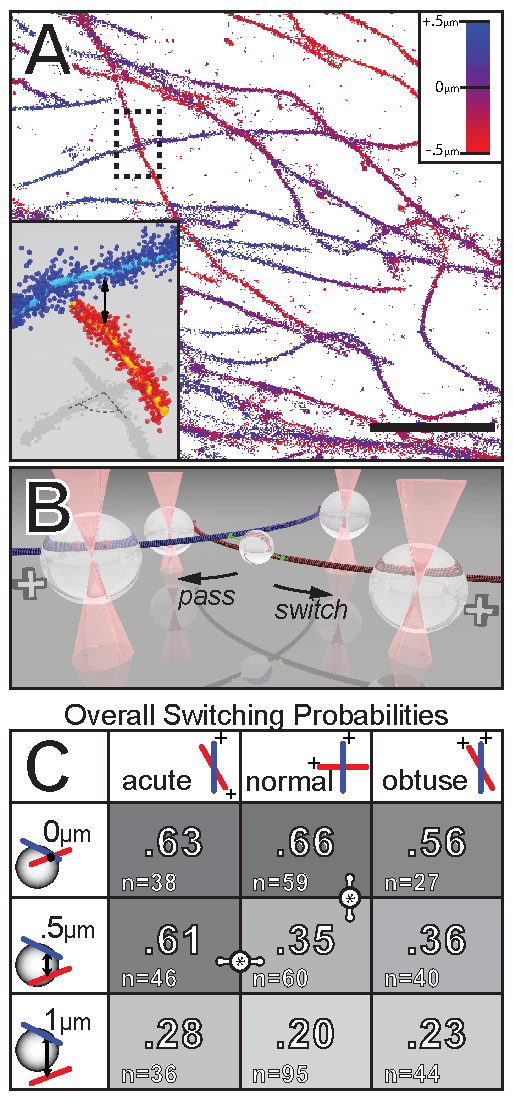
\includegraphics{project1/Fig_1FINAL}}
\end{figure}

The importance of MT cytoskeletal architecture is underscored by the fact that MT network remodeling occurs often in various diseases and during normal cellular processes. For example, neuritic de-arborization or restructuring is often encountered in neurodegenerative diseases \cite{VanBattum2015,DiPolo2015}. Microtubule remodeling is also observed in many neoplasias \cite{Parker2014} and is associated with pathways often disturbed in cancers \cite{Galmarini2003}. There is also evidence that suggests the geometry of the MT network, itself, acts as a regulator to tune insulin granule secretion in mouse pancreatic  $\beta$-cells \cite{Zhu2015}.
 
The cell can use multiple mechanisms to modulate its MT architecture. MTs can be locked in parallel \cite{Fink2009} or antiparallel \cite{Subramanian2010} alignment via cross-linking. Axonal branching generally shows a preference for normal angles \cite{Kalil2013}; low branch angles can arise from MT nucleating factors \cite{Petry2013}. The cell can set overall MT spacing by simply controlling the amount of polymerized tubulin, either via regulation of expression levels \cite{Dumontet1996} or filament stability \cite{Desai1997}. Filament spacing can also be controlled via MAPs that cross-link microtubules \cite{Hirokawa1988}. Microtubule and actin networks are often coupled and remodeling of one can drive structural changes in the other \cite{Chesarone2010,Young2008}. External factors which affect cell shape can also regulate MT network topology \cite{Gomez2016}. Finally, MT crossings are known to be special loci for intracellular regulation \cite{Hamant2013}. Currently, the implications of these topology variations for cargo logistics and overall biomechanics are not quantitatively understood.
 
Decoupling the influence of the MT network's 3D topology from regulatory protein factors is challenging. The same pathways that drive network remodeling can also couple to motor regulation. The result is that, to date, the impact of geometric changes in MT networks on intracellular cargo transport has been difficult to isolate and quantitate. It is common in biology to think in terms of chemical regulation. However, to truly understand how intracellular cargo transport functions, it is critical to gain a baseline understanding of how the 3D MT geometry alone impacts cargo distribution, starting at the most fundamental level of the MT network: individual MT-MT intersections.
Studying cargo navigational behavior as a function of 3D network geometry poses considerable experimental challenges. In vivo investigations cannot easily decouple chemical and topological regulation, as discussed above. Moreover, although theoretical work highlights its importance \cite{Erickson2013}, in vitro bead assays that use traditional MT-glass deposition techniques are also unable to model MT-MT crossings with controlled filament separation \cite{Ross2008,Vershinin2007}.
 
To address this question, we developed an in vitro system to suspend and dynamically manipulate multiple individual MT filaments in 3D. Each MT is manipulated individually via holographic optical trapping (HOT) of two or more bead handles (BH), as previously described \cite{Bergman2015}. We used this bottom-up approach to systematically construct MT-MT intersections featuring various angles and separations. We then measured the statistics of kinesin-1 driven model cargo (MC) transport on these model MT geometries, and used this data to constrain 3D simulations. We show from experimental data and theoretical analysis that navigational outcomes exhibit systematic variation based on 3D MT intersection geometry. Further, we propose dynamic mechanisms that explain the observed preferences.

\section{Results}

\subsection{Experimental Setup}

The broad aim of this work is to understand the impact of cytoskeletal geometry on intracellular transport. A comprehensive experimental model of all possible geometries (e.g. Fig \ref{fig:1}A) is well beyond the scope of any singular study, so we restricted our scope to representative model scenarios. We focused on the simplest type of intracellular MT intersections where just two filaments cross (Fig. \ref{fig:1}A, inset). We used silica microspheres, driven by full length KHC homodimers, as our MC. This is a common, albeit simplified, model for in vitro work. We chose to focus on assays outside the single-molecule regime because there is substantial evidence that
cargos in cells are often driven by multiple motor ensembles, and indeed multiple-motor ensembles are essential for a ToW to develop.

We used in vitro 3D MT manipulation via HOT \cite{Bergman2015} to examine three filament spacings: zero, radius, and diameter of the MC. Our MCs were \SI{1}{\micro\meter} in diameter, hence we constructed and observed MC transport across model intersections featuring 3 separation distances (\SI{0}{\micro\meter}, \SI{.5}{\micro\meter}, and \SI{1}{\micro\meter}). We decided to only parametrize this geometric range because the probability of a cargo interacting with both MTs for crossing separations greater than the cargo diameter quickly becomes negligible. For each separation distance, we examined three different angles of intersection, acute (MT polarities nearly counter aligned), normal (\SI{90}{\degree}), obtuse (MT polarities nearly aligned), for a total of nine geometric conditions.

We chose silica microspheres as our MCs because their density is 2.2x that of water. This biased the cargo to hang below the MT to which it was engaged, although Brownian motion along all three axes was both expected and observed. Thus, in our setup, we always deposited the MC (via HOT) onto the ``overpass" MT, such that the hanging cargo would be likely to encounter the lower, crossing MT (Fig. 1B). With this setup, our \SI{0}{\micro\meter} separation experiments resemble the ``underpass" MT geometry in prior crossing experiments, in which MTs were attached to a glass substrate \cite{Ross2008,Vershinin2007}. However, our experimental model allows for MT bending, twisting, and vibrations which cannot be recapitulated when MTs are firmly attached to a solid substrate. The absence of the solid glass substrate in our work is a major difference since the cargo can explore many more three-dimensional paths as it negotiates the intersection.

\subsection{Final navigational outcomes depend on 3D geometry}

For each of the nine MT network arrangements in our assays, we quantified final cargo routing outcomes strictly in terms of, ``switching" or ``passing", because detachment at intersections was negligible. In addition, we do not report pause events, because we can characterize the entire navigational event, even in cases where the MC navigational choice takes several seconds to make. Below, we report switching probability only, as passing probability is complementary.

Our results suggest that 3D MT network topology alone can be an effective regulator of cargo routing (Fig. \ref{fig:1}C). Geometries in the upper left corner of the table promote switching while those in the lower right corner promote passing. Therefore, routing outcomes are determined by multiple geometric factors interacting in non-trivial ways. Disentangling these factors by intuition alone is challenging, therefore we relied upon \textit{in silico} modeling. Helpfully, many fine mechanistic details are resolved by our experimental approach (see below), which constrain the \textit{in silico} model.

\subsection{Characterization of Tug-of-War events}

A cargo that does not engage in a ToW, does not switch; hence precisely distinguishing between ToW and non-ToW events is critical to dissect the mechanisms that lead to differential switching probabilities. Our spatiotemporal resolution is sufficient not only to establish whether a ToW took place, but also to precisely determine ToW durations.

We can readily identify ToW start and end by observing significant MC displacements away from MT axes and associated MT deflections (Fig. \ref{fig:2}A). MC tracks for representative pass (Fig. \ref{fig:2}B), and switch (Fig. \ref{fig:2}C) events are shown, along with their displacements projected along the axes of the intersecting MTs. A ToW start can be identified with the beginning of a sustained displacement upon the crossing MT's axis. ToW end can then be identified when the cargo snaps back upon dissociation from either the primary or crossing MT. BH displacements can also be used as an indicator of a ToW because the MC motors engaged in a ToW will exert force on the MTs that ultimately displaces the BHs (Fig. \ref{fig:1}B, \ref{fig:2}A \textit{middle}, D).

\begin{figure}
\centering
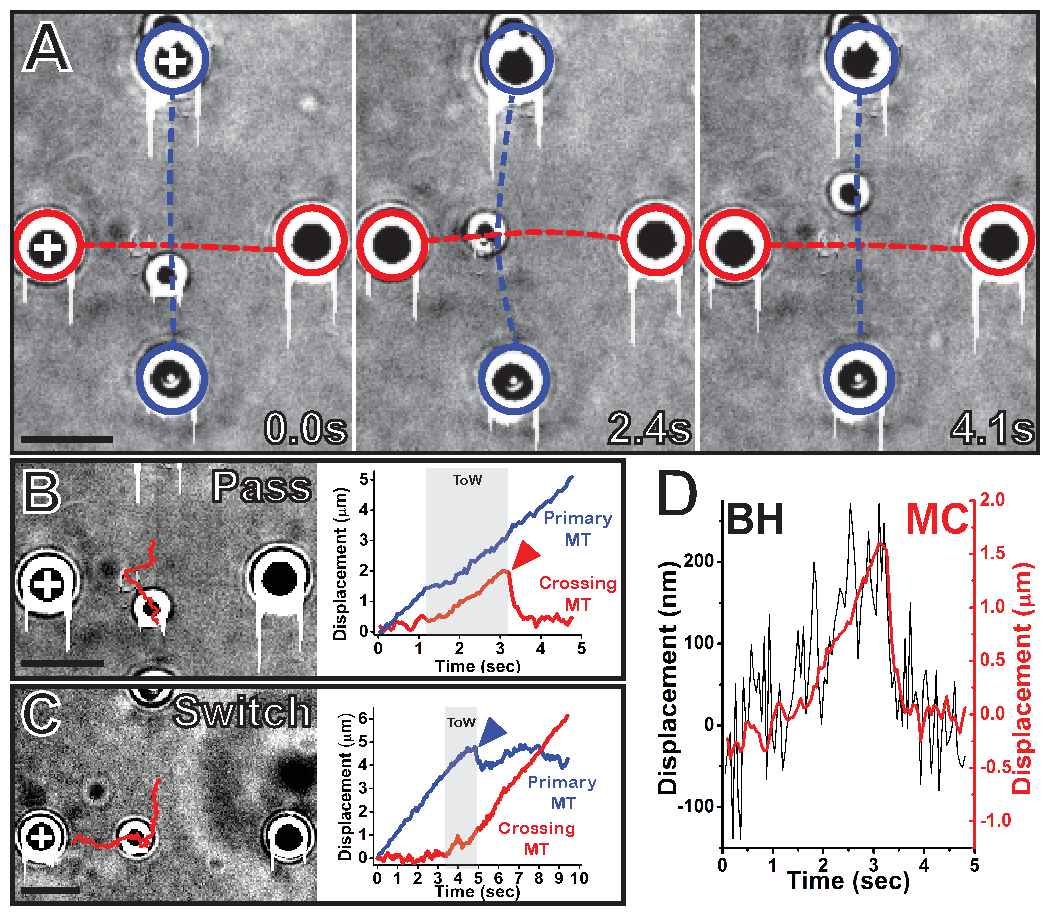
\includegraphics[scale=.7]{project1/Fig_2FINAL}
\caption[Identification and quantification of ToW]{Identification and quantification of ToW. \\
\textbf{(A)} Three video frames: before, during, and after ToW (left to right). Circles show BH
positions in the left panel and are positioned identically in middle and right panels. Dashed lines highlight positions of MTs inferred from video for each frame. Blue and red color scheme represents over- and underlying components respectively (\SI{.5}{\micro\meter} separation). Displacement of the top BH relative to its fiducial circle indicates presence of ToW (middle panel); its original position is restored once ToW has ended (right panel). White plus signs indicate the MT plus ends. Frame timings shown in lower right corner. \\
\textbf{(B)} Analysis of the pass event shown in panel (A). Left panel: Trajectory of MC (red) overlaid on one cropped video frame. Right panel: MC displacements projected along the primary (blue) and crossing (red) MT directions. Red arrowhead highlights the snapback event which is typical of a ToW conclusion. Gray band: ToW temporal extent ($\sim$ 1.9 s). \\
\textbf{(C)} Analysis of a switch event. Left panel: Trajectory of MC (red) overlaid on one video frame. Right panel: MC displacement projected along the primary (blue) and crossing (red) MT's axes (\SI{.5}{\micro\meter} separation). Blue arrowhead highlights when the MC undergoes a ``snapback", an event which is typical of a ToW conclusion. Gray band: ToW temporal extent ($\sim$ 1.6 s). \\
\textbf{(D)} MC displacement along the crossing (red) MT axis shown in (B) overlaid onto trace of BH displacement from trap center, due to ToW (for the top BH in (A)). All scale bars are \SI{5}{\micro\meter}.}
\label{fig:2}
\end{figure}

Although BH displacements can help confirm ToW presence and duration, their greatest benefit is that they are an indicator of how many motors were exerting force on the bead. We set the trap stiffness at $\sim$\SI{1}{\pico\newton}/\SI{100}{\nano\meter}, so that a single kinesin motor could not pull the BH out of the trap (escape event) but two or more motors working together could do so readily (Fig. \ref{fig:BHforce}). Quantifying collective activity of multiple motors via trap escape forces is a well-established approach both in vivo \cite{Ashkin1990,Gross2002} and in vitro \cite{McKenney2010} and has been validated in silico \cite{McKenney2010}. This setup allowed us to control the surface density of motors on MCs by discarding assays in which BH escape fraction exceeded 25\% of total events. This provided refined control on top of the more crude and variable approach of controlling motor concentration at incubation time. It also provided confidence that ToWs in our assays were dominated by forces from 1-2 kinesin motors; more motors are likely engaged on the MT but not all are positioned to exert force during the ToW.

\begin{figure}
\centering
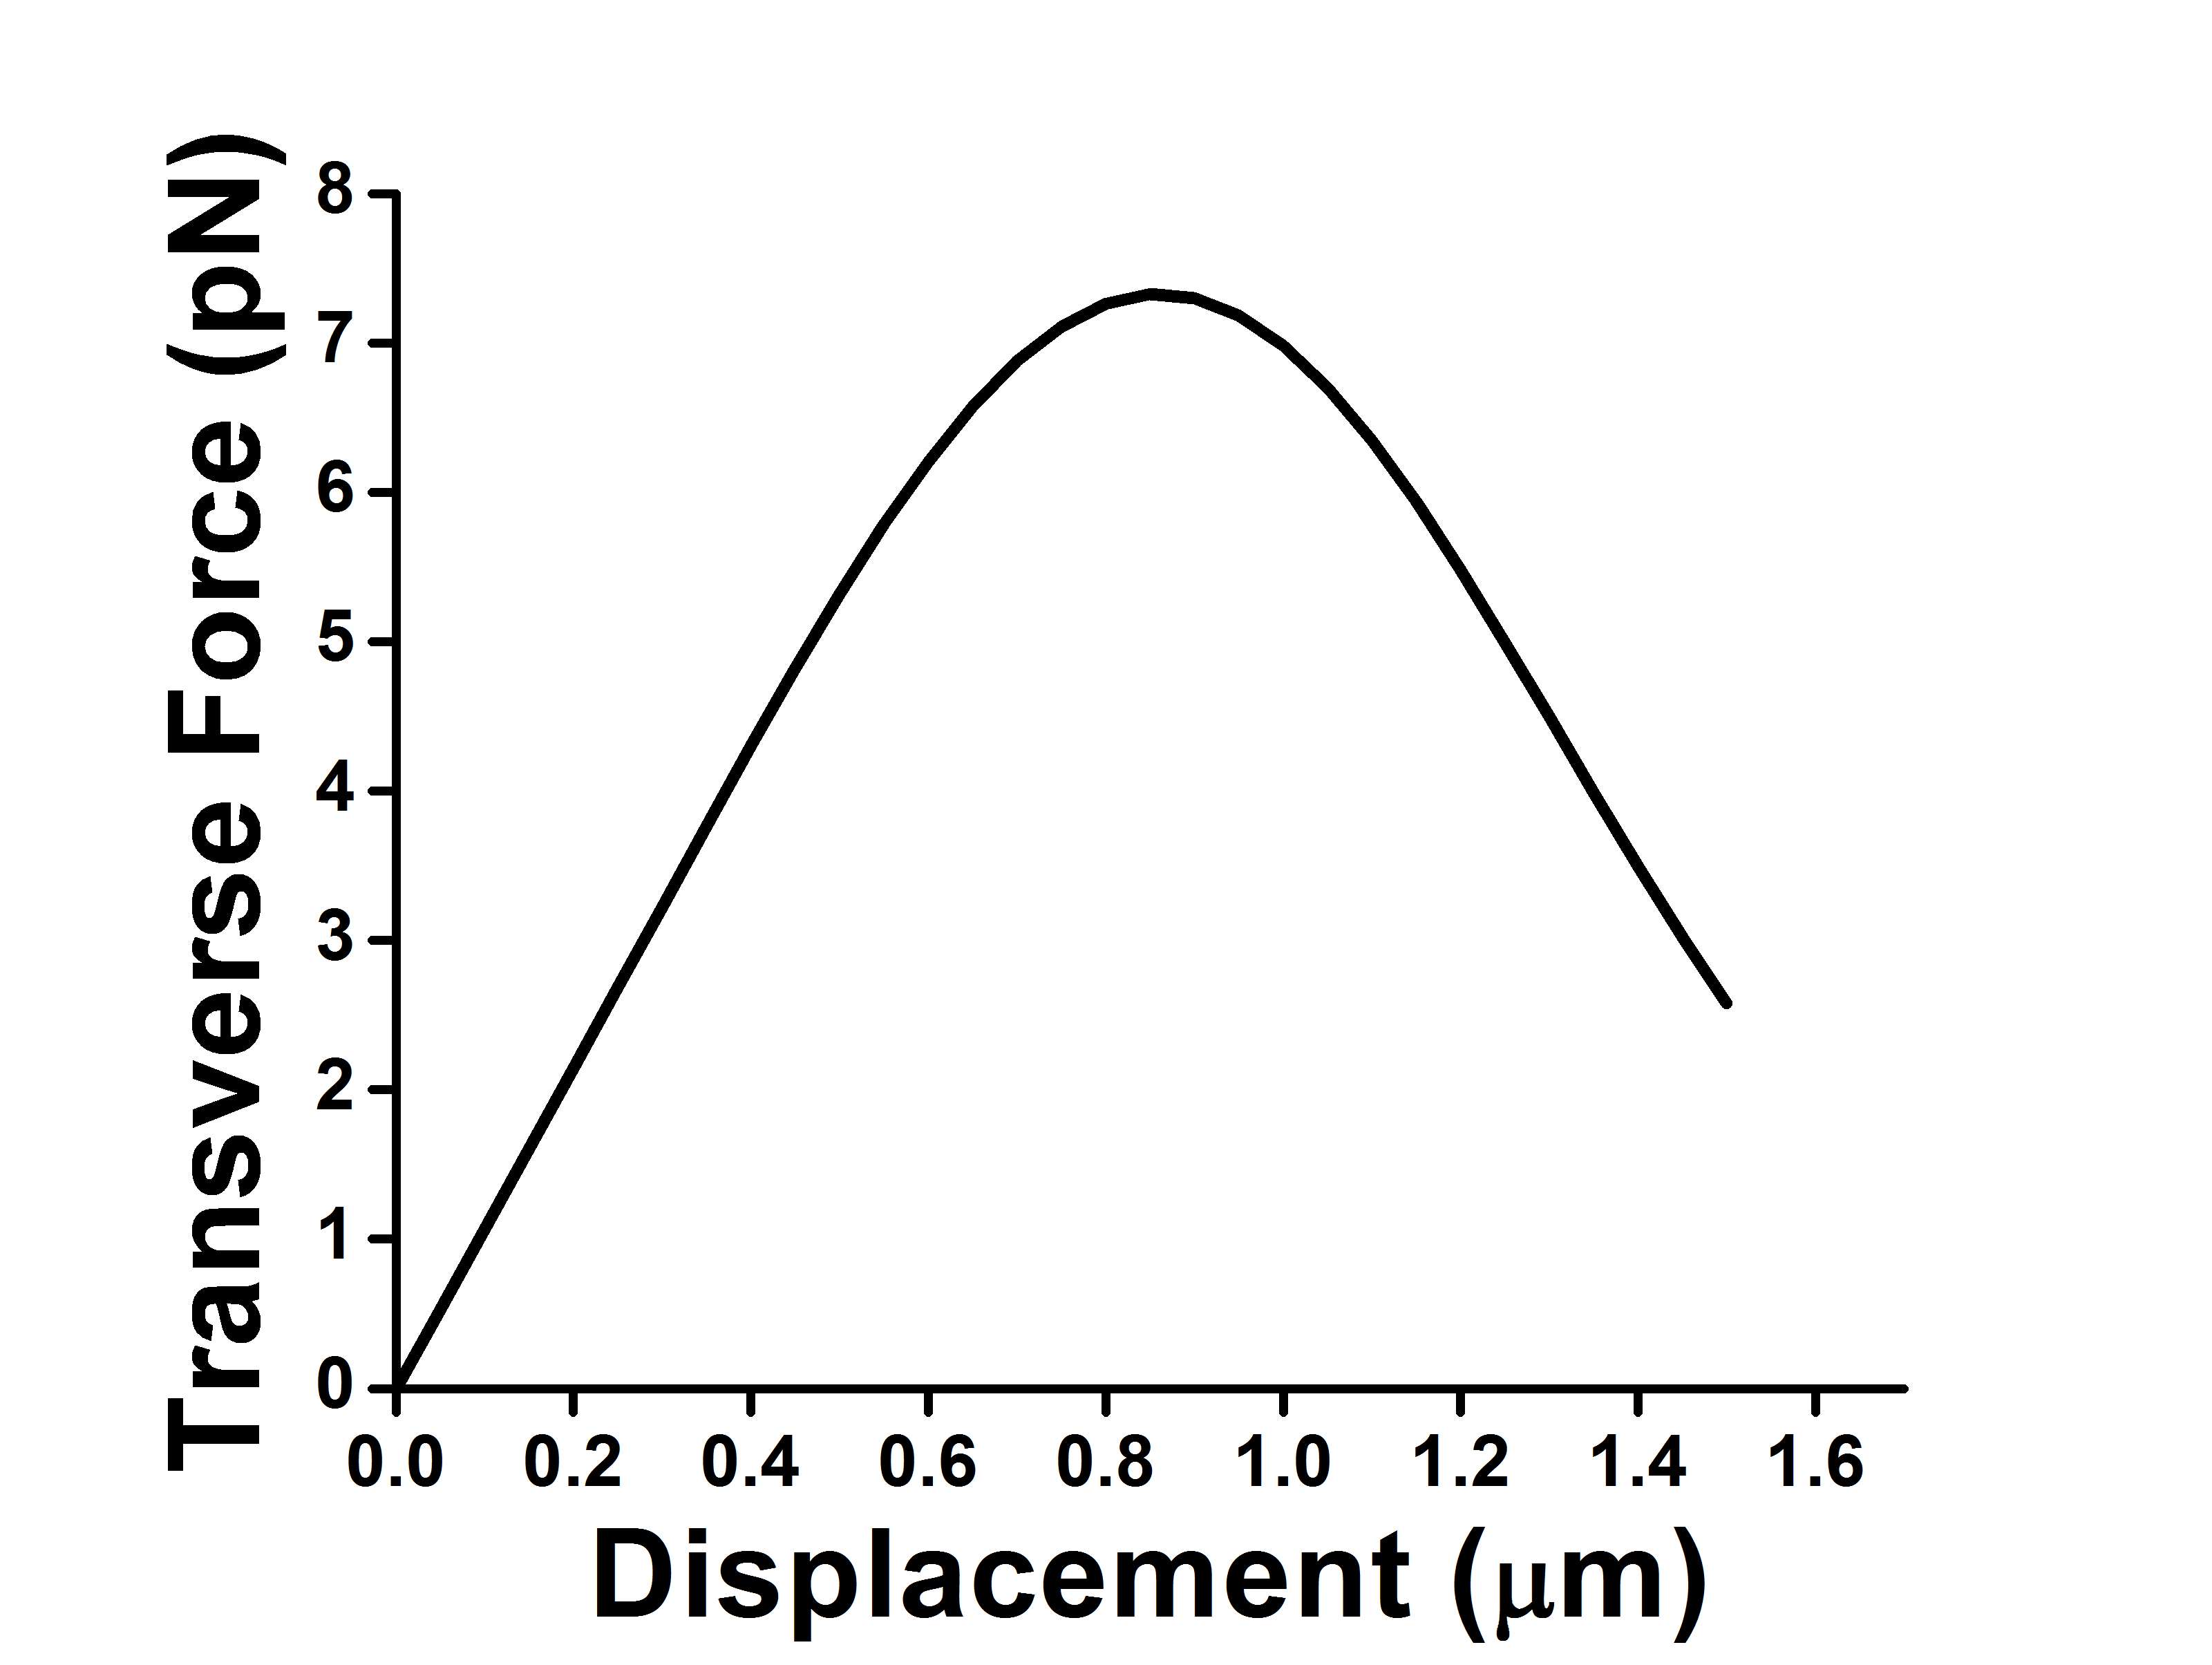
\includegraphics[width=4in]{FvsL}
\caption[Restoring force on Bead Handles]{Restoring force on a glass bead (index of refraction 1.55, \SI{1000}{\nano\meter} radius) exerted by the HOT for various displacements from trap center. Calculations were performed using previously published software\cite{Nahmias2002}.}
\label{fig:BHforce}
\end{figure}

\subsection{Mechanisms of cargo routing}

The ability to sensitively detect ToW events allowed us to quantify their probability. We could then also examine the probability for the cargo to pass or switch, conditional on ToW occurrence. This analysis is informative because these probabilities reveal different aspects of cargo dynamics (Fig. \ref{fig:3}). Our data indicates that ToW probability is sensitive to 3D geometry: it is higher for narrower filament separations, and for acute/obtuse angles (Fig. \ref{fig:3}A). For \SI{0}{\micro\meter} separations, ToW probability is so high that significant differences as a function of angle may not be practical to measure. A different pattern of navigational outcomes emerges when trivial passes (no-ToW events) are omitted (Fig. \ref{fig:3}B vs Fig. \ref{fig:1}C). Four out of nine geometries show switch probabilities close to 50\%. We also record switch probabilities that are significantly higher than 50\% for the following geometries: \SI{0}{\micro\meter} normal, \SI{0}{\micro\meter} acute, and \SI{.5}{\micro\meter} acute (p $<$ .05 Barnard's test). We conclude that geometric constraints can promote or inhibit switching outcomes for ToW events.

\begin{figure}
\floatbox[{\capbeside\thisfloatsetup{capbesideposition={right,top}}}]{figure}[\FBwidth]
{\caption[Cargo navigation flow chart, with associated outcome probabilities]{Cargo navigation flow chart, with associated outcome probabilities. \\
\textbf{(A)} Probabilities of ToW, as a function of 3D MT network geometry. \\
\textbf{(B)} Probabilities of switching conditional on ToW taking place, as a function of 3D MT network geometry. ** indicate probability is significantly higher than 50\% (p$<$0.05, Barnard's test).} \label{fig:3}}
{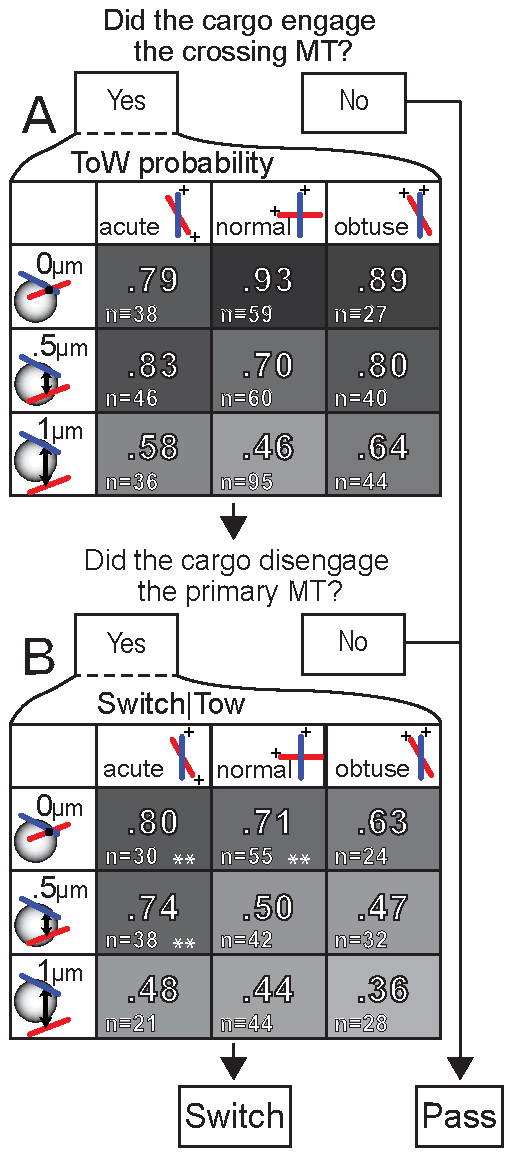
\includegraphics{project1/Fig_3FINAL}}
\end{figure}

\subsection{A mathematical model of cargo transport reproduces observed switch probabilities}

As mentioned above, it is difficult to disentangle the mechanism through which each factor acts to (in concert) determine ToW and switching probabilities. Therefore, to gain further insight into the mechanism determining cargo routing, we constructed an \textit{in silico} model of cargo transport. This model allows us to examine experimentally unobservable details, such as how motor locations, bound states and force states change with time.

The model incorporates relevant experimental details including: the well-established properties of kinesin-1 motors, and cargo translational and rotational diffusion, however, simulated MTs do not move, twist, or bend (Fig. \ref{fig:4}A). 500 cargo trajectories were simulated independently for each assay geometry, and probabilities of ToW and switching were then determined analogously to the experimental data. For full simulation details and parameter fitting procedure, see \ref{description} and \ref{sec:simulation}. Briefly, there were two parameters that could not be established from current experiments or prior literature: average motor number attached to MCs and each motor's on-rate. These two parameters were constrained by matching three experimental observations: ToW probability as a function of geometry (Fig. \ref{fig:ToW_fit}), fraction of BH escape events and MC run lengths (Fig. \ref{fig:run_length_fit}). Thus, the model is fully constrained and therefore predictive.

We found good agreement between experimentally observed and theoretically predicted probabilities of ToW'ing and switching (Fig. \ref{fig:4}B-D). We now turn to investigation of the quantitative details of ToW and switching (next two sections), and their implications for the mechanisms of cargo navigation at MT intersections.

\begin{figure}
\centering
\includegraphics[width=\linewidth]{project1/Fig_4FINAL}
\caption[Mathematical model of navigational outcomes]{Mathematical model of navigational outcomes. \\
\textbf{(A)} Snapshots of simulated cargo activity at an intersection (color coding as in Fig. \ref{fig:3}).
Examples of Pre-ToW, ToW, and post-TOW states are shown (left, middle, right respectively). Motors bound to the primary MT are shown in cyan. Motors bound to the crossing MT are shown in magenta. Unbound motors are shown as green spherical protrusions from MC; sphere radius represents motor's maximal reach. Bead's ``prime meridian" demarcated to emphasize rotational movement.
\textbf{(B)} Simulated probabilities to engage in ToW. Probability of undergoing ToW for each geometry is shown as thin symbols (error bars: SEM). Experimental data is shown as large symbols (error bars: 95\% C.I.). Experimental data points for \SI{.5}{\micro\meter} geometries shifted slightly horizontally to aid the eye.
\textbf{(C)} Simulated probability to switch, given the cargo engaged in ToW. Simulated and experimental data represented as in (B).
\textbf{(D)} Simulated probability to switch, overall, i.e. the product of probability to ToW (B), and probability to switch, given ToW (C). Simulated and experimental data represented as in (B).
\textbf{(E)} Snapshot of a ToW for \SI{0}{\micro\meter}, \SI{90}{\degree} geometry. Here, primary MT motors are blocked from passing the intersection by the crossing MT at \SI{0}{\micro\meter}. Bound and unbound motors represented as in (A).
\textbf{(F)} Probability to switch increases with increasing simulated fluid viscosity. Error bars: SEM.
\textbf{(G)} Force exerted by crossing MT on the cargo for \SI{.5}{\micro\meter} geometries (mean $\pm$ SEM).}
\label{fig:4}
\end{figure}

\subsection{The influence of intersection geometry on ToW probability}

The longer a cargo spends within reach of the primary and intersecting MTs (henceforth, the ToW zone), the more chances unbound motors on the cargo have, to engage the intersecting MT. This phenomenon can be understood from a simple, heuristic model. If we consider the cargo as having a single rate of binding to the crossing MT given by $k_{\text{on}}^\text{macro}$, the probability the cargo binds to the crossing MT before leaving the ToW zone is given by 
\begin{equation} \label{eq:rate_war_main}
p(\text{ToW})=\frac{k_{\text{on}}^\text{macro}}{k_{\text{on}}^\text{macro} +  v / d_\text{ToW} },
\end{equation}
where $v$ is the cargo velocity and $d_\text{ToW}$ is the length of the ToW zone. This simple model can accurately reproduce experimental ToW probabilities for both the \SI{.5}{\micro\meter} and \SI{1}{\micro\meter} separation distance geometries (Fig. \ref{fig:heuristicEXP}), but not for the \SI{0}{\micro\meter} separation geometries. This strongly suggests that there are mechanisms at play for \SI{0}{\micro\meter} separations which are not present at other distances (see below).

\begin{figure}
\centering
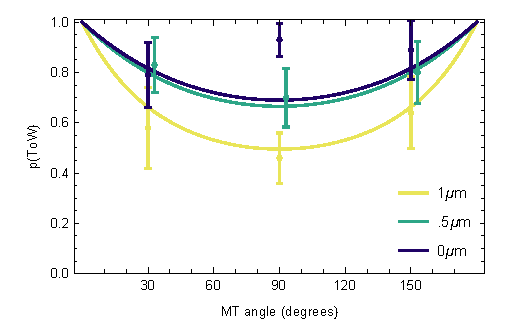
\includegraphics[width=12cm]{heuristicEXP.pdf}
\caption[Solutions to the heuristic model for ToW probability]{Solutions to the heuristic model for ToW probability \\
A heuristic model (given in equation \ref{eq:rate_war_main}) poses the probability of undergoing ToW as the the probability of the cargo binding (with constant binding rate) to the crossing MT before leaving the ToW zone (see equation \ref{eq:ToW_zone} and figure \ref{fig:heuristic}). 
%Solutions to the model reproduce qualitative features of the simulated ToW probability for \SI{.5}{\micro\meter} and \SI{1}{\micro\meter} separation distances, shown in main text figure 4. The fact that the heuristic model does not qualitatively reproduce ToW probabilities for \SI{0}{\micro\meter} geometries highlights the importance of steric effects at these geometries. 
Solutions shown as solid curves. Bars represent 95\% confidence intervals for corresponding experimental data. Bars for data at \SI{.5}{\micro\meter} shifted slightly to aid the eye. Solutions plotted with $k_\text{on}^\text{macro}$ set to \SI{1}{\per\second}.
} \label{fig:heuristicEXP}
\end{figure}

On the other hand, our full model closely recapitulates all experimental ToW probabilities, including \SI{0}{\micro\meter} separation data. It is encouraging that the model captures several \textit{a priori} intuitive features of the system. For \SI{0}{\micro\meter} geometries, if a cargo is driven by multiple motors then there is guaranteed to be a pool of motors able to bind the crossing MT (namely, the already engaged motors). Thus, we \textit{a priori} expect the ToW probability for all angles to be close to 1, which our model reproduces. For \SI{.5}{\micro\meter} and \SI{1}{\micro\meter} geometries, we expect higher ToW probability for longer ToW zones (acute and obtuse angles). Indeed, simulated ToW probabilities were smallest for \SI{90}{\degree} intersections (Fig. \ref{fig:4}B). Also, as expected, they were symmetric about the normal angle (since kinesin binding is not affected by MT polarity). Simulated ToW probabilities also increased when MT separation decreased from \SI{1}{\micro\meter} to \SI{.5}{\micro\meter}, as expected. When the intersecting MT encounters the MC's midsection, at \SI{.5}{\micro\meter} separations, it samples more of the bead's surface area (especially when rotational diffusion is taken into account). Hence, at \SI{.5}{\micro\meter} separation, more motors are given a chance to engage on the crossing MT, which increases ToW probability.

\subsection{The influence of intersection geometry on navigational outcomes, given ToW}

Experimentally, we observe a large range of geometries (most \SI{.5}{\micro\meter} and \SI{1}{\micro\meter} geometries) where the conditional probability to switch is $\sim$50\%. At first glance, this appears to be a relatively intuitive result: if ToW lasts $\sim$\SI{1}{\second} or more (our experimental ToW durations average $\sim$\SI{3}{\second}, Fig. \ref{fig:ToWtimes}), then the motor team engaged on the crossing MT should be able to reach steady state \cite{Erickson2011}, and become equal in number to the primary motor team. With two equivalent ways to proceed, the probability of either choice would indeed be $\sim$50\%. However, such a consideration is too simplistic as we discuss below.

\begin{figure}
\centering
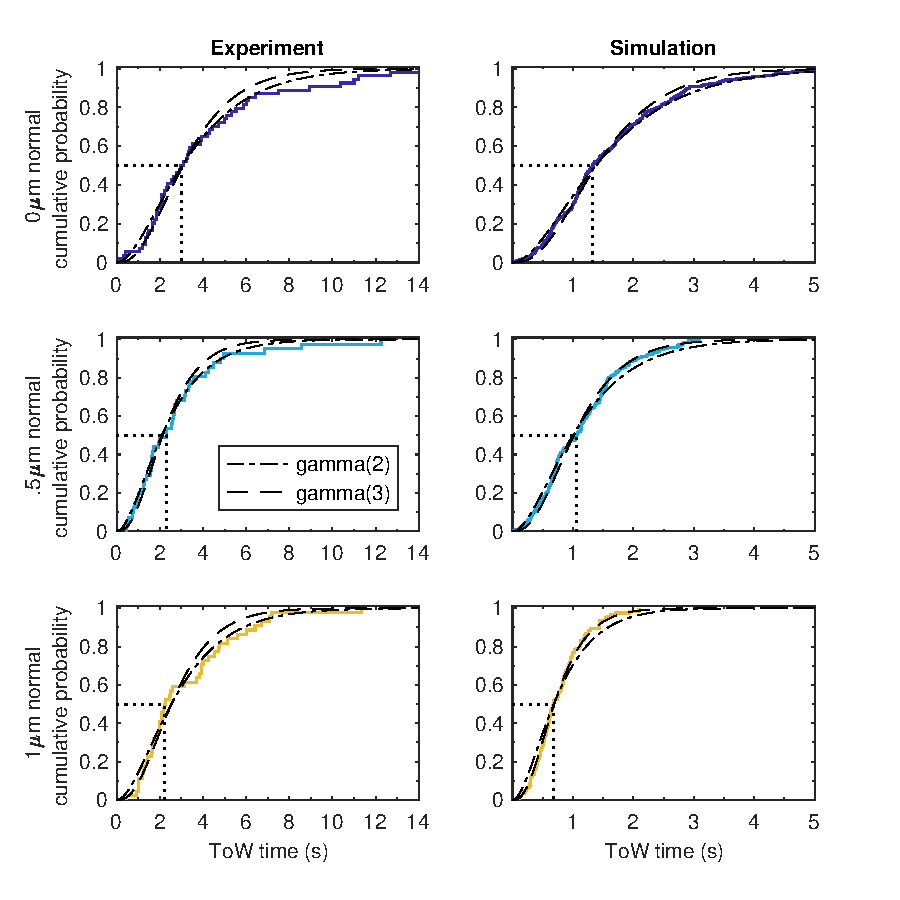
\includegraphics[width=6in]{ToWtime_fits.pdf}
\caption[Empirical cumulative probability distributions for ToW times]{Empirical cumulative probability distributions for ToW times \\
The time for which cargos underwent ToW in 90 degree (normal) geometries was measured in experiments and simulations. Cumulative distributions are shown for each geometry. To aid interpretation, medians are highlighted with dotted lines. Fits to gamma cumulative distribution functions are shown in dashed lines. Good fits to gamma distributions with shape parameter 2-3 indicate distributions are well approximated as generated from 2-3 independent exponential events which we interpret as motor unbinding events.
} \label{fig:ToWtimes}
\end{figure}

Experimental results allow for sensitive identification of ToW, so that ToW events can be analyzed separately from trivial ``no-ToW" intersection passages (Fig. \ref{fig:3}). The same analysis can be performed for simulated events (Fig. \ref{fig:4}B-D). A careful analysis of the simulations helps us shed light on the mechanistic details of cargo navigation.

We first assessed whether the number of motors in the two ensembles is in fact equal in our simulations. We find that contrary to na\"ive expectation, the number of engaged motors on the secondary MT is comparable but consistently lower than that on the primary MT (ratio of $\sim$0.7; Fig. \ref{fig:num_engagedEXP}). The reason is that the motors already engaged on the primary MT constrain the bead from full range of linear and rotational diffusion. Once a ToW starts, the bead diffusion is even more constrained; this curtails the number of motors that can reach the secondary MT. Thus, the team of motors pulling along the primary MT generally has an advantage. However, the two paths to proceed are not equivalent either. The crossing MT itself can serve as an obstacle for bead progress and exert a force which hinders the MC from passing (Fig. \ref{fig:4}G). The smooth decrease from passing to switching prevalence across our experimental geometries (Fig. \ref{fig:3}B) therefore reflects the balance between net motor activity (which is biased in favor of moving along the primary MT) and steric hindrance from the crossing MT.

\begin{figure}
\centering
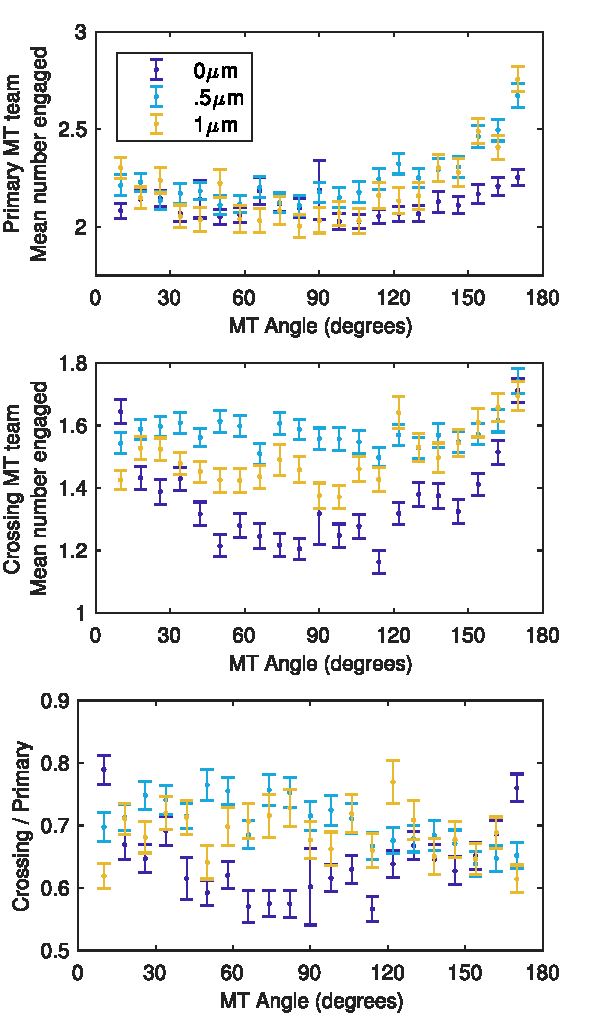
\includegraphics[width=4in]{num_engagedEXP.pdf}
\caption[Number of motors engaged on MTs during ToW]{ Number of motors engaged on MTs during ToW\\
The mean number of motors engaged on the primary (\textit{top}) and crossing (\textit{center}) MTs during simulated ToWs are shown for each geometry. Additionally, the ratio of the mean number of motors engaged on the crossing MT to the mean number engaged on the primary MT is shown (\textit{bottom}). Data are represented as mean +/- SEM. Separation distances are colored as specified in the legend in the top panel.
} \label{fig:num_engagedEXP}
\end{figure}

\subsection{The limits of geometric regulation}

Our results establish that a single MT intersection can significantly bias cargo routing towards more switching or more passing. Can a single MT intersection produce a near 100\% bias for switching or passing? What are the mechanisms which affect these limits? It is easy to see that $\sim$100\% passing naturally occurs for intersections with filament separation much greater than MC diameter. Is 100\% switching attainable? To address this, we consider two special cases which lead to elevated probability to switch, and their broader implications for geometric regulation. For completeness, we also discuss each experimental geometry individually in \ref{sec:results}.

\subsection{Low filament separations}

A closer look at the geometric setup (Fig. \ref{fig:4}E) makes it clear that the \SI{0}{\micro\meter} case is qualitatively distinct. At \SI{0}{\micro\meter} separation, the crossing MT sterically hinders the motors engaged on the primary MT, but not for the MC itself. To pass, the cargo can ``hurdle" over the crossing MT due to Brownian motion but this is improbable for our large silica MCs (density $\approx$ 2.2x water). Hurdling would also be unlikely in the viscous cytosolic environment (even for smaller cargos). The only other way to pass is by a mechanism we refer to as ``monkey-barring." To pass via monkey-barring, the MC must first diffuse underneath the crossing MT so that some of the unengaged motors on its surface could bind to the distal side of the primary MT (Fig. \ref{fig:5}A). The motors proximal to the crossing MT must then gradually disengage. The above suggests that passing at \SI{0}{\micro\meter} separation should have a sensitive dependence on the diffusion properties of the medium. This is indeed seen in our simulations (Fig. \ref{fig:4}F). In fact, for viscosities close to intracellular range, where cargo diffusion is suppressed, the preference to switch approaches 100\%.

\begin{figure}
\centering
\includegraphics{project1/Fig_5FINAL}
\caption[Mechanisms that elevate switch probabilities]{Mechanisms that elevate switch probabilities.\\
\textbf{(A)} Illustration of MC approaching a normal intersection with a separation of \SI{0}{\micro\meter}. \\1) Motors engaged on the primary MT can detach, then rebind to the crossing MT. \\2) Unengaged motors can bind the crossing MT. \\3) Unengaged motors can bind the primary MT at a site distal to filament intersection - the first step in the monkey-barring mechanism. \\All motors are in green regardless of engagement status.\\
\textbf{(B)} Illustration of MC engaged in ToW at an acute \SI{.5}{\micro\meter} intersection. A minimal ToW with only two motors is shown for visual clarity. The forces exerted by motors are counter aligned (grey arrows) and serve to wedge the MC between the MTs. Red arrows point to MT plus ends.}
\label{fig:5}
\end{figure}

\subsection{Acute angles / intermediate separations}

Why is switching more prevalent for \SI{.5}{\micro\meter} acute geometry? Again, this must be due to the crossing MT acting as a strong hindrance, but the mechanism cannot be the same as in the previous section. Here, monkey-barring is not feasible but hurdling is. Evidently, in this case, for switching probability to be elevated, hurdling must be suppressed. The vertical forces associated with the ToW for \SI{.5}{\micro\meter} acute geometry pull the MC between MTs. This effectively wedges the cargo between the two MTs, which indeed prevents hurdling. We refer to this mode of steric hindrance as ``chop-sticking" (Fig. \ref{fig:5}B). Note that in our simulations, MTs were not allowed to bend, which would likely be a factor under experimental conditions. In reality, the two motor teams engaged in a ToW during chop-sticking would be expected to pull the two MTs closer together, which would make the crossing MT an even stronger obstacle to passing. This is likely the reason why experimentally observed switching probability for \SI{.5}{\micro\meter} acute geometry is somewhat higher than theoretical prediction.

\section{Discussion}

Cargos driven by multiple motors can exhibit incredibly complex behavior. Even when one considers this for a single cargo moving along a single MT, the system complexity is sufficient to lead to highly non-trivial emergent behaviors \cite{Kunwar2008,Jamison2010}. The number of motors in biologically relevant systems is typically small which necessitates highly detailed experiments and modeling to account for not only averaged behavior but also the effect of fluctuations. The addition of just one more filament adds such complexity that the emergent behaviors can dramatically diverge to give rise to discrete outcomes: passing and switching. It is therefore a fascinating model system to study emergent behaviors in biology.

We have modeled this problem in a highly controlled experimental environment in which we imposed very specific restrictions on cargo size and other experimental variables. We then performed highly detailed modeling of our system \textit{in silico} to generalize our experimental results. We were thus able to infer the key processes which underlie our observations. This enables us to extrapolate how cargo routing might function in cells (and other environments).

Our analysis shows that the team of motors driving the cargo along the primary MT is generally at an advantage, even when the ToW is prolonged. This implies that there is an inherent bias to pass. However, our data shows that for many geometric conditions passing and switching is balanced, and in some cases, switching dominates. The missing factor which shifts the balance between passing and switching is the extent to which the crossing MT acts to sterically hinder the motors progressing along the primary MT.

We show that the crossing MT can indeed be an effective obstacle, especially when it intersects at an acute angle with intermediate separation, or near-zero separation. Both types of geometries significantly inhibit passing but via different mechanisms: intermediate separations with acute angles lead to chop-sticking, while near-zero filament separations mean that passing is only accessible by means of monkey-barring (which is an unlikely event). These results imply that the cell could selectively route cargos of different sizes by controlling MT intersection angle and spacing.
Our simulations closely follow the experimental results but two important deviations are seen: the conditional probability to switch given that ToW already started is higher in experiments than in simulations. Also, the time a cargo spends at the intersection is higher in the experiment than in simulation (Fig. \ref{fig:ToWtimes}). In both cases, the discrepancy is clearly linked to the fact that we model MTs as an infinitely rigid rod. To date, MT rigidity has been mostly studied separately from MT-based transport. Our work suggests that MT bending and more generally biomechanics of the MT cytoskeleton must be taken into account in future studies of intracellular motility as they are a non-negligible contributor to cargo routing.
                      
A faithful and detailed \textit{in silico} model of cargo motility and the ToW process enables us to then speculate about cargo navigation patterns beyond our specific conditions. First, we show that if viscosity increases, then switching would be further favored for near-zero filament separations. In effect, our simulations lead us to speculate that not only MT geometry but also local microrheology can be a regulator of cargo routing.

We also predict that extremely short motors should find reaching across the crossing MT for near-zero separations particularly difficult, so cargos driven by very short motors would preferentially switch at intersections. It is tempting to speculate that overall kinesin length evolved to reduce the probability of cargos getting trapped in filament-filament switching loops.

On a more architectural level, our results suggest that for each cargo type and size there is a critical MT density at which efficient transport can be inhibited by too much switching at intersections. This prediction from the single molecule level dove-tails with the more qualitative observations for the insulin secretion process \cite{Zhu2015}.

Our work opens many new directions for future work, including studies of more complex intersections, more complex cargos and motor complexes. Together these baseline studies can then serve as a basis for studying chemical regulation of motility in the context of cytoskeletal network geometry. A gradual from-the-bottom-up increase in complexity can then gradually lead to comprehensive quantitative understanding of intracellular cargo fluxes, from a single-molecule mechanistic perspective.

\section{Materials and Methods:}

\subsection{Optical trapping and 3D motility experiments:}

Our holographic optical trapping and bead assays were performed as previously described \cite{Bergman2015}. However, in present work, enzymatically dead KIF5A heavy chain dimers were adsorbed onto bead handles non-specifically. Switch/pass outcomes were assessed live during the experiments from the video feed and recordings were conducted until definitive outcome was attained. Video records of bead positions were tracked using custom software (MATLAB, MathWorks, Natick, MA).

\subsection{Super-resolution imaging:}

African green monkey kidney epithelial (BSC1) cells were labeled with primary antibody, alpha-tubulin, against microtubules followed by secondary antibody labeling with Alexa Fluor 647. Super-resolution images were recorded with a Vutara commercial microscope (Bruker, Salt Lake City, UT) based on the single molecule localization (SML) biplane FPALM technology \cite{Juette2008,Mlodzianoski2009}.

Microtubules were imaged using a 647 nm excitation laser, and 405 nm activation laser in photoswitching buffer comprising of 20 mM cysteamine, 1\% betamercaptoethanol, and oxygen scavengers (glucose oxidase and catalase) in 50mM Tris+10 mM NaCl+10\% glucose buffer at pH 8.0. Images were recorded using a 60x/1.2 NA Olympus water immersion objective and Photometrics Evolve 512 EMCCD camera with gain set at 50, frame rate at 50 Hz and maximal powers of 647 nm and 405 lasers set at 8 and 0.05 kW/cm$^2$ respectively.

Data was analyzed by the Vutara SRX software (version 6.00). Single molecules were identified by their brightness frame by frame after removing the background. Identified particles were then localized in three dimensions by fitting the raw data in a customizable region of interest (typically 12x12 pixels) centered around each particle in each plane with a 3D model function which was obtained from recorded bead data sets. Fit results were stored as data lists for further analysis.

\subsection{Statistical analysis:}

Much of our data is in the form of contingency tables. Barnard's exact tests were used to assess significance of differences between outcomes.

\subsection{Simulations:}

See Chapter \ref{sec:model}.

\section{Acknowledgements:}

We are grateful Dr. Erik Jorgensen for helpful discussions and guidance on super-resolution imaging of microtubules. This work was supported by NSF grant number ENG-1563280 to M.V., NIH T32 EB009418-07 to M.B. and NIH R01 GM123068 to J.A. and S.G.
\chapter{Discussion}

The results detailed in the previous two chapters describe how specific cargos, engineered outside of the cell, navigate intersections between two microtubules, also constructed outside the cell.
This study adds to previous \textit{in vitro} work on cargo routing at intersections, which described the ability of cargos to switch between microtubules at intersections constructed by laying microtubules on top of each other \cite{Ross2008}.
This work adds to our understanding of how cargos switch microtubules by extending into three dimensions.
Doing so necessitated the development of sophisticated new experimental methods by the Vershinin lab, by which the position of two microtubules can be controlled relative to each other with high precision.
This was achieved by using holography to create and individually manipulate several optical traps \cite{Bergman2015}.
Using this technique, we were able to find that intersection geometry can influence cargos to switch or pass.
We find that the same cargos have as much as a 2/3 chance of switching in some geometries, while they have as low as a 1/5 chance in other geometries.

To help understand why intersection geometry has a strong influence on switching probability we used a computational model.
We based the model on basic physics and the well-known \textit{in vitro} behavior of the molecular motors used in the experiments.
The model allowed us to learn that routing outcomes can be understood through a balance between the steric hinderance of the crossing microtubule, which influences cargos to switch, with the stronger motor team on the primary microtubule, which influences cargos to pass.
The geometry of the intersection dictates how strongly steric hinderance affects the cargo.

The cell interior is significantly more complex than our experiments or simulations.
The cytoplasm is highly visco-elastic for intracellular cargos \cite{Guo2014,Ahmed2018}.
Both kinesin and dynein motors are often present on cargos \cite{Gross2004,Hancock2014}, along with a host of other molecules which regulate their activity (e.g. \cite{Reddy2016}).
Microtubules are adorned with many molecules thought to regulate the workings of the motors in different ways \cite{Yu2015,Sirajuddin2014}.
In the face of this complexity, what does our study add to the understanding of how cargos are directed in the cell?

First, it establishes that geometry alone can influence cargo routing.
Regulation of transport is often thought about through the lens of molecular specificity --- how molecules which are present on a cargo change transport properties.
This result points out physical size of the cargo and intersection angle as important properties for cargo routing, which are independent of the molecules present.
As a result, the cell could route cargos of different sizes in different ways even if the molecules that decorate them are identical.

Second, while the experiments and modeling were done in a simplified situation, the explanation we find for why the results are the way they are is not specific to the particular case we examine.
Microtubules will pose a steric hinderance to cargos moving in the cell.
How much hinderance depends on the rigidity of the cargo, pointing to a possible role for cargo rigidity in routing. 
Since we identified the stronger motor team on the primary microtubule as an important factor in determining routing outcomes, we can infer that different motor organizations on the surface of the cargo may modulate this effect.
Therefore setting motor organization might be a method for the cell to control cargo routing.

Third, it establishes baseline behavior. We now understand there is significant complexity in switching behavior with just one type of motor and two microtubules which are identical in all but their spatial location. The cell might decorate microtubules with other molecules or modify microtubule surfaces to help it control intersection navigation. This work is a first step toward understanding how modifications which change the behavior of individual molecular motors can influence navigation.

In the future, we hope to expand on this work in several ways. We are interested in assaying the navigation outcomes of organelles purified from cells. The Gross lab has the ability to purify lipid droplets \cite{Reddy2016}, which could be assayed for switching in a similar way to the \textit{in vitro} engineered cargos in this work. We are also interested in understanding how various microtubule associated proteins (such as Tau, on which the Vershinin and Gross labs have worked previously \cite{Vershinin2007}) may modulate switching probabilities. 

% These commands fix an odd problem in which the bibliography line
% of the Table of Contents shows the wrong page number.
\clearpage
\phantomsection

% "References should be formatted in style most common in discipline",
% abbrv is only a suggestion.
\bibliographystyle{abbrv}
\bibliography{background/background,project1/project1,appendix1/appendix1}

% The Thesis Manual says not to include appendix figures and tables in
% the List of Figures and Tables, respectively, so these commands from
% the caption package turn it off from this point onwards. If needed,
% it can be re-enabled later (using list=yes argument).
\captionsetup[figure]{list=yes}
\captionsetup[table]{list=yes}

% If you have an appendix, it should come after the references.
\appendix
%\documentclass[onecolumn]{article}

%define margins
%\usepackage[margin=1in,top=1.0in, left=1in,right=1in]{geometry}

%core packages
%\usepackage{siunitx} %for writing numbers with units vis \SI, \num
%\usepackage{amsmath} %for cases, multline environments
%\sisetup{detect-weight=true, detect-family=true}
%\usepackage{physics} %for \vqty, \dd, \dv
%\usepackage{graphicx} %for \includegraphics
%\usepackage{enumitem} %for indenting items in description environment
%\usepackage{caption}

%\usepackage[final]{changes} %for keeping track of edits
%\definechangesauthor[name={Matt Bovyn},color=blue]{MB}
%\definechangesauthor[name={Jun Allard},color=orange]{JA}

%for nicer Tau
%\usepackage{ upgreek }
%\renewcommand{\tau}{{\,\uptau}}

%citations with biblatex
%for S prefix, need input argument defernumbers=true
%then before \printbibliography need a \newrefcontext[labelprefix=S]
%\usepackage[backend=biber,defernumbers=true]{biblatex}
%\addbibresource{suppliment.bib}

%some citations from Mendelay don't play well with the default ascii encoding
%use utf8 instead
%\usepackage[utf8]{inputenc}    % utf8 support       %!!!!!!!!!!!!!!!!!!!!
%\usepackage[T1]{fontenc}       % code for pdf file  %!!!!!!!!!!!!!!!!!!!!

%to change the figure and table labels to S#
%\setcounter{table}{0}
%\renewcommand{\thetable}{S\arabic{table}}
%%\setcounter{figure}{0}
%\renewcommand{\thefigure}{S\arabic{figure}}

%\usepackage{authblk}

%bring in convenience commands
\input appendix1/preamble.tex

%\usepackage{hyperref}%for links, should always come last

%\begin{document}

%\title{Supplemental information for \\ Cargo navigation across 3D microtubule intersections}
%\date{}
%\author[a,1]{Jared Bergman}
%\author[b,c,1]{Matthew Bovyn}
%\author[d]{Manasa Gudheti}
%\author[b,c,e]{Steven Gross}
%\author[b,c,f,2]{Jun Allard}
%\author[a,g,h,2,3]{Michael Vershinin}
%\affil[a]{Department of Biology, University of Utah}
%\affil[b]{Department of Physics and Astronomy, University of California, Irvine}
%\affil[c]{Center for Complex Biological Systems, University of California, Irvine}
%\affil[d]{Visiting Scientist, Department of Biology, University of Utah}
%\affil[e]{Department of Developmental and Cell Biology, University of California, Irvine}
%\affil[f]{Department of Mathematics, University of California, Irvine}
%\affil[g]{Department of Physics and Astronomy, University of Utah}
%\affil[h]{Center for Cell and Genome Science, University of Utah}
%\affil[1]{JB and MB contributed equally to this work}
%\affil[2]{JA and MV contributed equally to this work}
%\affil[3]{To whom correspondence should be addressed. Email: vershinin\{at\}physics.utah.edu}

%\maketitle

%\newpage

%Contents: \\
%\begin{enumerate}[label=\arabic*,leftmargin=*,labelsep=2ex,ref=\arabic*]
%    \item[] Supplemental figures
%      \begin{enumerate}[label*=.\arabic*,leftmargin=*,labelsep=2ex]
%        \item[] Figure S1: Restoring force on BH \dotfill 3
%        \item[] Figure S2: Solutions to the heuristic model for ToW probability \dotfill 4
%        \item[] Figure S3: ToW times \dotfill 5
%        \item[] Figure S4: Mean motors engaged during ToW \dotfill 6
%      \end{enumerate}
%    \item[] Mathematical model of cargo dynamics
%      \begin{enumerate}[label*=.\arabic*,leftmargin=*,labelsep=2ex]
%        \item[] 1 Model description \dotfill 7
%        \item[] 2 Numerical simulation of the model \dotfill 11
%        \item[] 3 Model Results \dotfill 15
%      \end{enumerate}
%     \item[] Captions for supplemental movies \dotfill 22
%     \item[] Supplemental references \dotfill 23
%\end{enumerate}

%\newpage


\chapter{Mathematical Model for Routing at Intersections} \label{sec:model}

The following is adapted from a manuscript created by Jared Bergman, Matthew Bovyn, Manasa Gudheti, Steven Gross, Jun Allard and Michael Vershinin. The project was initiated by Michael Vershinin. Michael Vershinin and Jared Bergman developed the experiments. Cargo navigation experiments were performed by Jared Bergman. Manasa Gudheti performed super-resolution microscopy. The model was created by Matt Bovyn, Steve Gross, and Jun Allard. Matt Bovyn wrote and performed simulations. The model was modified and developed to fit the experimental situation by Matt Bovyn with advice from Jun Allard, Steve Gross, Jared Bergman and Michael Vershinin.

Matt Bovyn and Jun Allard wrote the description of the model and model results, included as this chapter. The manuscript was published as \cite{Bergman2018}, and the materials in this chapter became the supplementary information.
%\vspace*{2\baselineskip}
%\centerline{\textbf{\LARGE Mathematical model of cargo dynamics}}
%\vspace{4\baselineskip}

%%%%%%%%%%%%%%%%%%%%%%%%%%%%%%%%%%%%%%%%%%%%%%%%%
\section{Model description} \label{description}

We present a three dimensional mesoscale model for the dynamics of the cargo, which takes into account rotational and translational diffusion, as well as stochastic stepping and binding of the motors. The locations of the cargo bead and motors attached to it are governed by a set of stochastic ordinary differential equations. Binding state and location of the motor head along the microtubule (MT) are considered discrete states and transitions between them occur stochastically, modeled as Poisson processes. We construct a Monte Carlo numerical simulator, based on a hybrid Euler-Maruyama-Gillespie scheme, and simulate an ensemble of stochastic trajectories, from which we  derive probabilities for tug of war and switching.

Motors in the model have two states:
\begin{description}[labelindent=\parindent,font=\normalfont]
\item[Bound:] A motor $i$ is defined by two points: one represents the the motor domains, which we call the head $\vec{h}^i$; the other represents the location at which the motor is bound to the bead, which we call the anchor $\vec{a}^i$. The motor has a rate of stepping along the MT $\kstep^i$ and a rate of unbinding from the MT $\koff^i$.
\item[Unbound:] A motor $i$ is defined by one point, the anchor location $\vec{a}^i$. The motor has a rate of binding to MT $j$, $\kon^{i,j}$, that depends on its location relative to the MT as described below.
\end{description}
We track the anchor locations, head locations of bound motors, the location of the cargo center $\vec{c}$, and the cargo orientation $\vec{\theta}$.

%**************************************************************************************************************
\subsection{Stochastic ordinary differential equations for cargo motion}

\begin{figure}
\centering
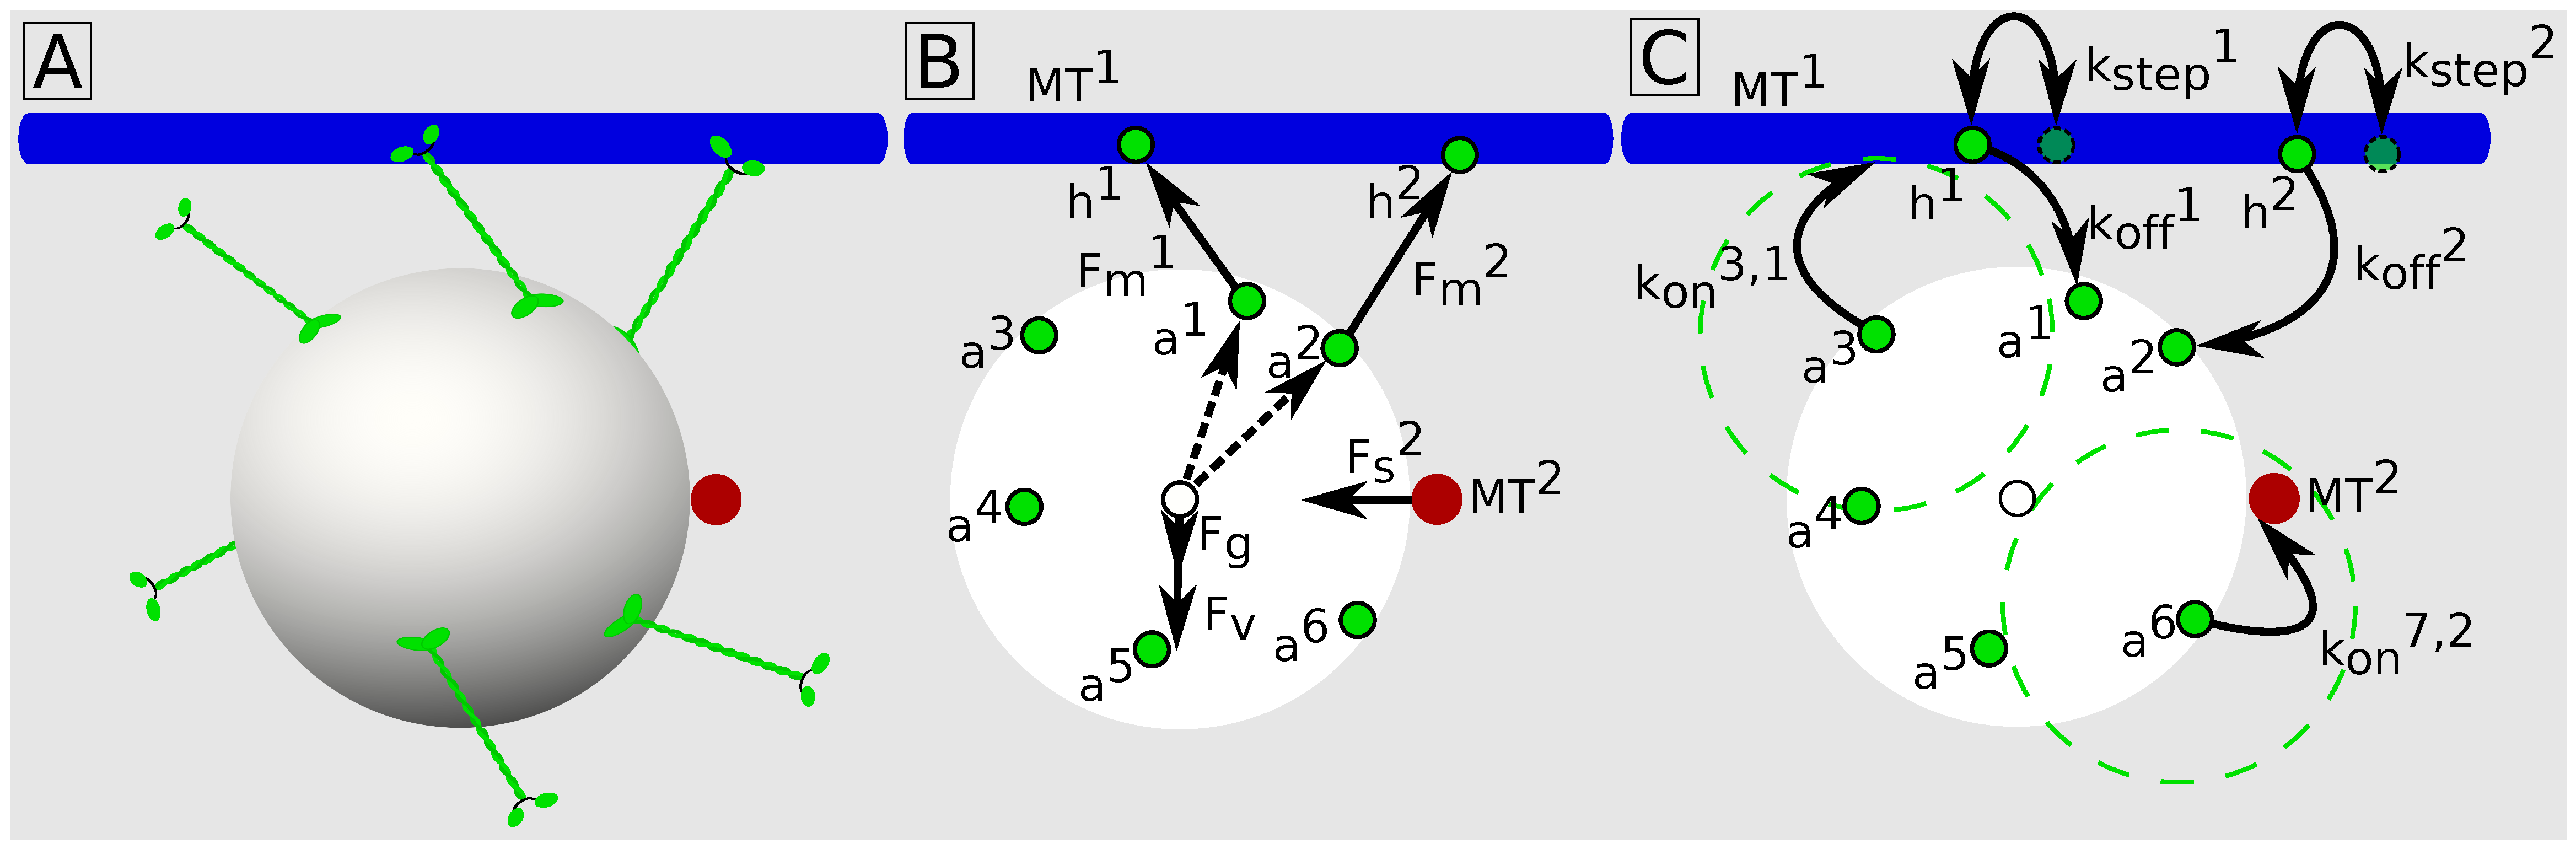
\includegraphics[width=6.5in]{appendix1/diagrams.eps}
\caption[Diagrams of simulated cargo dynamics]{Diagrams of cargo dynamics \\
A) Schematic of a model cargo in motion. Kinesin motors are shown in green, primary MT in red, crossing MT in blue, and bead in white. \\
B) Free body diagram of the cargo corresponding to the cartoon in A. Anchor locations $\vec{a}^i$ and head locations $\vec{h}^i$ are shown with green dots. Cargo center location $\vec{c}$ is shown with a white dot with black outline. Forces are shown with solid arrows. Dashed arrows show the lever arm through which the motor forces exert torque. \\
C) Diagram showing the possible state changes corresponding to the cartoon in A. Unbound motors have on rates greater than 0 if their anchor is less than 1 motor length from a MT. Bound motors have rates of stepping and unbinding.
} \label{fig:FBD}
\end{figure}

We first impose force-balance on the cargo. The motion of the cargo is the inertialess regime (Reynolds number $\sim 10^{-6}$), so we omit the inertia term. A free body diagram showing the deterministic forces acting on model cargo is shown in figure \ref{fig:FBD}B. All forces must balance, so
\begin{equation} \label{eq:forcebalance}
\sum \vec{F} = \underbrace{\sum_i \vec{F}_m^i}_{\text{motor forces}} + \underbrace{\sum_j \vec{F}_s^j}_{\text{steric forces}} + \underbrace{\vec{F}_g}_{\text{force of gravity}} + \underbrace{\vec{F}_b}_{\text{Brownian force}} + \underbrace{\vec{F}_v}_{\text{viscous force}} = 0.
\end{equation}
Similarly, we can write the balance of torques on the model cargo
\begin{equation} \label{eq:torquebalance}
\sum \vec{\tau} = \underbrace{\sum_i \vec{\tau}_m^i}_{\text{torque from motor forces}} +\underbrace{\vec{\tau}_b}_{\text{Brownian torque}} + \underbrace{\vec{\tau}_v}_{\text{viscous torque}} = 0.
\end{equation}
By specifying the forms of each of these forces below, we construct the equations of motion of the cargo center $\vec{c}$ and cargo orientation $\vec{\theta}$.

%------------------------------------------------------------------------------------------------------------------------------
\subsubsection*{Motor forces}

We model the force that the motor exerts on the cargo as originating from the stretch in spring-like motor stalks, based on experimental measurements \cite{Kojima1997,Jeney2004} and in line with  previous models \cite{Erickson2011,Korn2009,Kunwar2008}. The form of this force is that of a one-way (tension-only) spring with rest length equal to the length of the motor. The force $\vec{F}_m^i$ exerted by motor $i$ on the cargo bead is given by
\begin{equation} \label{eq:motor_spring}
\vec{F}_m^i \left( \vec{a}^i,\vec{h}^i \right) = 
\begin{cases}
	- \kappa_m \left( \left| \vec{h}^i - \vec{a}^i \right| - L \right) \left( \frac{\vec{h}^i - \vec{a}^i}{\left| 		\vec{h}^i - \vec{a}^i \right|} \right) & \left| \vec{h}^i - \vec{a}^i \right| >  L\\
	0 & \text{otherwise}
\end{cases}.
\end{equation}
This force also exerts a torque on the cargo bead, given by the cross product of the lever arm and force vector
\begin{equation} \label{eq:motor_torque}
\vec{\tau}_m^i \left( \vec{a}^i,\vec{h}^i,\vec{c} \right)= 
\left( \vec{a}^i - \vec{c} \right) \times \vec{F}_m^i \left( \vec{a}^i,\vec{h}^i \right).
\end{equation}

%------------------------------------------------------------------------------------------------------------------------------
\subsubsection*{Steric forces}


The cargo bead and MTs are prevented from overlapping in space by a steric force with the form of a one-way (compression-only) spring, given for MT $j$ by 

\begin{equation} \label{eq:steric_force}
\vec{F}_s^j(\vec{c})= 
\begin{cases}

	- \kappa_s \left(R - \vqty\Big{ \rvec{\vec{c}} } \right) \left( \frac{\rvec{\vec{c}}}{\vqty\big{ \rvec{\vec{c}} }} \right) & \vqty\Big{ \rvec{\vec{c}} } <  R\\
	
	0 & \text{otherwise}
	
\end{cases},
\end{equation}
where $\rvec{\vec{p}}$ is a vector from point $\vec{p}$ to the nearest point on the MT. This is found by computing the perpendicular distance from $\vec{p}$ to the MT surface, given by
%formula for vector from point to center of MT
\def\ceq{\left( \xmt^j-\vec{p} \right) - \left( \left( \xmt^j - \vec{p} \right) \cdot \dmt^j \right) \dmt^j}
%shortcut for R_MT/ceq because I want the parentheses to be the same size
\def\rbyceq{\frac{R_\text{MT}}{\vqty\bigg{\ceq}}}
%
\begin{multline} \label{eq:r_vec}
\rvec{\vec{p}} = 
\left( 1- \rbyceq \right)  \\
\left( \ceq \vphantom{\rbyceq} \right).
\end{multline}

%------------------------------------------------------------------------------------------------------------------------------
\subsubsection*{Force of gravity}

The experimental system uses a silica bead with density greater than water as the cargo. Therefore the model cargo experiences a small but significant force due to gravity given by the buoyancy of the bead,
\begin{equation} \label{eq:F_g}
\vec{F}_g= \frac{4}{3} \pi R^3 (\rho_b - \rho_w) \vec{g},
\end{equation}
where $\rho_b$ and $\rho_w$ are the mass densities of the silica bead and water, respectively.

%------------------------------------------------------------------------------------------------------------------------------
\subsubsection*{Brownian force}

The Brownian force $\vec{F}_b$ is a random variable with mean 0 and variance $2 k_B T \xi$, where $\xi$ is the drag coefficient and $k_B T$ is the thermal energy unit. Specifically,
\begin{align} \label{eq:Brownian_force}
\ev{\vec{F}_b} &= \vec{0} \\
\ev{\vec{F}_b(t) \cdot \vec{F}_b(s)} &= 2 (k_B T) (6 \pi \eta R) \delta(t-s)
\end{align}
where we have inserted the translational drag coefficient of a sphere at low Reynold's number and $\delta(x)$ is the Dirac delta function.

Similarly, the Brownian torque on the bead is a random variable characterized by
\begin{align} \label{eq:Brownian_torque}
\ev{\vec{\tau}_b} &= \vec{0} \\
\ev{\vec{\tau}_b(t) \cdot \vec{\tau}_b(s)} &= 2 (k_B T)(8 \pi \eta R^3) \delta(t-s).
\end{align}

%------------------------------------------------------------------------------------------------------------------------------
\subsubsection*{Viscous force}

In the low Reynolds  limit, linear drag dominates. The drag on the cargo is thus given by Stokes' Law,
\begin{equation} \label{eq:trans_drag}
\vec{F}_v=-6 \pi \eta R \dv{\vec{c}(t)}{t}.
\end{equation}
The viscous torque is given by the rotational analogue to Stokes' Law,
\begin{equation} \label{eq:rot_drag}
\vec{\tau}_v=-8 \pi \eta R^3 \dv{\vec{\theta}(t)}{t}.
\end{equation}

%------------------------------------------------------------------------------------------------------------------------------
\subsubsection*{Construction and discretization of the stochastic ordinary differential equations}

With the forms of forces known, we  rewrite equations \ref{eq:forcebalance} and \ref{eq:torquebalance} as a pair of coupled ordinary stochastic differential equations
\begin{equation} \label{eq:cSDE}
\dv{\vec{c}(t)}{t} = 
%
\frac{1}{6 \pi \eta R} \left( 
\sum_i \vec{F}_m^i \left( \vec{a}^i(t) ,\vec{h}^i(t) \right) + 
\sum_j \vec{F}_s^j(\vec{c}(t)) + 
\vec{F}_g 
\right) + 
%
\frac{1}{6 \pi \eta R} \vec{F}_b(t)
\end{equation}
and
\begin{equation} \label{eq:thetaSDE}
\dv{\vec{\theta}(t)}{t}=
%
\frac{1}{8 \pi \eta R^3} \left( 
\sum_i \vec{\tau}_m^i \left( \vec{a}^i(t) ,\vec{h}^i(t) ,\vec{c}(t) \right) 
\right) + 
%
\frac{1}{8 \pi \eta R^3} \vec{\tau}_b(t),
\end{equation}
Equation \ref{eq:cSDE} is a specific implementation of the overdamped Langevin equation, used in Brownian dynamics. Equation \ref{eq:thetaSDE} is its rotational counterpart.

We discretize these equations according to the Euler-Maruyama method. For an update from the $n$th timestep at time $t_n$ to the next time $t_{n+1}$ with $\Delta t \equiv t_{n+1}-t_n$, the discretization is
\begin{multline} \label{eq:cSDE_discretized}
\vec{c}(t_{n+1}) = \vec{c}(t_n) +
\frac{1}{6 \pi \eta R} \left( \sum_i \vec{F}_m^i \left( \vec{a}^i(t_n) ,\vec{h}^i(t_n) \right) + \sum_j \vec{F}_s^j(\vec{c}(t_n)) + \vec{F}_g \right) \Delta t \\
+ \sqrt{2 \frac{k_B T}{6 \pi \eta R} \Delta t} \;\vec{G}_c(t_n)
\end{multline}
and
\begin{equation} \label{eq:thetaSDE_discretized}
\vec{\theta}(t_{n+1})= \vec{\theta}(t_n) +
\frac{1}{8 \pi \eta R^3} \left( \sum_i \vec{\tau}_m^i \left( \vec{a}^i(t_n) ,\vec{h}^i(t_n) , \vec{c}(t_n) \right) \right) \Delta t + \\
\sqrt{2 \frac{k_B T}{8 \pi \eta R^3} \Delta t} \;\vec{G}_\theta(t_n).
\end{equation}
%where $\vec{G}_c^n = \begin{pmatrix} G_1^n \\ G_2^n \\ G_3^n \end{pmatrix}$ is vector of three independent gaussian random variables with mean \num{0} and variance \num{1}, characterized by $\expval{G_\alpha(n) G_\beta(n')} = \delta^{\alpha\beta} \delta^{n n'}$, with $\alpha$ and $\beta$ denoting any pair of cartesian coordinates and $n$ and $n'$ denoting any pair of time steps
where $\vec{G}_c^n$ and $\vec{G}_\theta^n$ are two mutually uncorrelated vectors of three independently and identically distributed gaussian random variables with mean \num{0} and variance \num{1}.

%------------------------------------------------------------------------------------------------------------------------------
\subsubsection*{Update of anchor locations}

Since the motors are statically bound to the bead, the change in their locations is fully defined by the change in the location of the center of the bead $\vec{c}(t_{n+1})-\vec{c}(t_n)$ and the change in the orientation of the bead $\vec{\theta}(t_{n+1}) - \vec{\theta}(t_n)$.

The change in the bead orientation $\vec{\theta}(t_{n+1}) - \vec{\theta}(t_n)$ corresponds to a vector pointed along the axis of rotation of the bead with a length corresponding to the magnitude of the rotation in radians. This vector can be converted into a rotation matrix $\mathbf{M}_R(t_n)$. The next location of anchor $i$ is then calculated by finding
\begin{equation} \label{eq:anchor_update}
\vec{a}^i(t_{n+1})=\vec{a}^i(t_n) + \left( \vec{c}(t_{n+1})-\vec{c}(t_n) \right) + 
\left( \mathbf{M}_R(t_n) \left( \vec{a}^i(t_n) - \vec{c}(t_n) \right) + \vec{c}(t_n) \right).
\end{equation}

%**************************************************************************************************************
\subsection{Poisson processes}


We model all state transitions in the system as Poisson processes, diagrammed in figure \ref{fig:FBD}C. Experiments have reported exponential distributions of times between steps \cite{Carter2005} and times before unbinding \cite{Kunwar2011}. This is also the most basic assumption we can make for times before binding.

%\begin{figure}
%\centerline{\includegraphics[width=5cm]{CTMC.jpg}}
%\caption{Continuous time Markov chain diagram} \label{fig:CTMC}
%\end{figure}

%------------------------------------------------------------------------------------------------------------------------------
\subsubsection*{Stepping}

Kinesin motors step processively along MT tracks in a hand-over-hand fashion, with each motor domain taking \SI{16}{\nano\meter} steps \cite{Yildiz2004} that move the center of mass of the motor forward by \SI{8}{\nano\meter} \cite{Svoboda1993}. The rate at which the motor steps, and thus the motor velocity, depends on the load the motor is stepping against in a way well modeled as 
\begin{equation} \label{eq:stepping}
\kstep^i = 
\begin{cases}
\frac{v}{d}\left(1-F_m^i/F_s \right)^w & F_m^i < F_s \\
0 & F_m^i \geq F_s
\end{cases},
\end{equation}
as described in \cite{Kunwar2010}.

When a motor steps, it is moved forward along the direction of the MT $j$ to which it is bound by the step distance $d$. This translates to an update of the head position 
\begin{equation} \label{eq:step_head}
\vec{h}^i(t_{n+1}) = \vec{h}^i(t_n) + d \left(\dmt^j \right).
\end{equation}

%------------------------------------------------------------------------------------------------------------------------------
\subsubsection*{Unbinding}

Kinesin unbinds from the MT with a rate dependent on the force experienced by the motor. Measurements have shown that unbinding rate increases exponentially below stall \cite{Milic2014}. Above stall, measurements have shown that unbinding rate increases only slowly with increasing force \cite{Kunwar2011}. Therefore, we state the unbinding rate as
\begin{equation} \label{eq:unbinding}
\koff^i = 
\begin{cases}
\epsilon_0 \exp(F_m^i/F_d) & F_m^i \leq F_s \\
a+b F_m^i & F_m^i>F_s
\end{cases}.
\end{equation}
When a motor unbinds, it is simply put into the unbound state as defined at the beginning of this section.

%------------------------------------------------------------------------------------------------------------------------------
\subsubsection*{Binding}

The conditions which govern the rate of binding to the MT are not well known. In the absence of detailed experimental elucidation, we make only the most basic assumptions possible: the motor domains must be able to reach the MT to bind, and, if this condition is met, the motor binds with a constant rate. This translates to an on rate for motor $i$ to MT $j$ given by
\begin{equation} \label{eq:binding}
\kon^{i,j} = 
\begin{cases}
\pi_0^{\text{micro}} & \abs{ \rvec{\vec{a}^i} } \leq L\\
0 & \text{otherwise}
\end{cases}
\end{equation}
where $\rvec{\vec{a}^i}$ is given by equation \ref{eq:r_vec}.

When a motor $i$ binds to MT $j$, the head location is placed at the location on the MT nearest the anchor location $\vec{a}^i$, given by 
\begin{equation} \label{eq:bind_head}
\vec{h}^i(t_{n+1})=\vec{a}^i(t_n) + \rvec{\vec{a}^i(t_n)}.
\end{equation}

%%%%%%%%%%%%%%%%%%%%%%%%%%%%%%%%%%%%%%%%%%%%%%%%%
\section{Numerical simulation of the model} \label{sec:simulation}

Section \ref{description} outlines a numerical scheme for updating for the model's dynamic variables in equations \ref{eq:cSDE_discretized}, \ref{eq:thetaSDE_discretized} and \ref{eq:anchor_update} over a timestep $\Delta t$. We simulate the model forward in time using these equations. Time steps are chosen dynamically. The largest stable time step for the Euler-Maruyama scheme is given by $\xi/\kappa$, where $\xi$ is the drag coefficient and $\kappa$ is the spring constant of the stiffest operating spring. The maximum time step is chosen based on the springs active during that step. The equivalent stiffness of multiple active motor springs is taken into account, but the steric spring in equation~\ref{eq:steric_force} remains by far stiffest in the system if it is active. 

For each timestep, we generate exponential random variables from distributions with means set by each Poisson rate, given in equations \ref{eq:stepping}, \ref{eq:unbinding}, and \ref{eq:binding}, as in the Gillespie (next-event) algorithm. If any of these times are smaller than the maximum stable time step, the smallest generated time is chosen. If the smallest generated time came from an unbinding rate, a state change is implemented at the end of the update step by setting the motor to the unbound state. If this time came from a stepping rate or binding rate, the update occurs by equation \ref{eq:step_head} or \ref{eq:bind_head}, respectively. If no generated time is shorter than the maximum stable time step, the update is done with the maximum stable time step and there is no state change. The memoryless property of the exponential distributions which underlie the Poisson processes ensure that these substeps do not change the overall dynamics.

The numerical simulation is written in C. It takes approximately \SI{.5}{\second} to simulate \SI{1}{\second} of cargo motion with a \SI{3.3}{\giga\hertz} Intel Core i5 processor (single thread).

%**************************************************************************************************************
\subsection{Model parameters}

The kif5A motors used in experiments are members of the well studied kinesin-1 family. As such,  many of the model parameters have been estimated in previous experiments. The parameters used to simulate the model are given in table \ref{tab:params}. There are two parameters in the model not well constrained by experiments in the literature: the number of motors on a cargo, $N$, and the on rate of a motor given that it is close enough to the MT to bind, $\pi_0^{\text{micro}}$.

\begin{table}
\begin{tabular}{p{.1\linewidth} p{.28\linewidth} p{.15\linewidth} p{.3\linewidth}} 
\hline Parameter & Description & Value & Notes \\ \hline

$N$ & Number of motors on the bead & \num{30} & Determined by fit to experiments in this paper \\

$\kappa_m$ & Kinesin stalk spring constant & \SI{320}{\pico\newton\per\micro\meter} & Measured in \cite{Kojima1997,Jeney2004}  \\

$L$ & Kinesin length & \SI{80}{\nano\meter} & Measured in \cite{Hirokawa1989,Scholey1989} \\

$\pi_0^{\text{micro}}$ & Base binding rate (microscopic) & \SI{10}{\per\second} & Determined by fit to experiments in this paper. Lower bound estimated in \cite{Leduc2004,Klumpp2005}\\

$\epsilon_0$ & Base unbinding rate & \SI{.7}{\per\second} & Estimated from run lengths \cite{Block1990,Milic2014,Li2016} \\

$a$ & Superstall unbinding rate intercept parameter & \SI{1.07}{\per\second} & Measured in \cite{Kunwar2011} \\

$b$ & Superstall unbinding rate slope parameter & \SI{.186}{\per\second\per\pico\newton} & Measured in \cite{Kunwar2011} \\

$F_s$ & Stall force & \SI{5}{\pico\newton} & Measured in \cite{Visscher1999,Kunwar2011,Milic2014} \\

$F_d$ & Critical detachment force & \SI{4}{\pico\newton} & Measured in \cite{Schnitzer2000,Kunwar2011,Milic2014} \\

$v$ & Unloaded motor velocity & \SI{1}{\micro\meter\per\second} & Velocities measured here \\

$d$ & Step size & \SI{8}{\nano\meter} & Measured in \cite{Svoboda1993} \\

$w$ & Curvature index & \num{2} & Measured in \cite{Visscher1999,Fallesen2011}  \\ \hline

$\kappa_s$ & Steric spring constant & \SI{40000}{\pico\newton\per\micro\meter} & Set high enough to ensure the cargo spends no more than 5 time steps in a row intersecting a MT \\

$R$ & Cargo bead radius & \SI{.5}{\micro\meter} & Provided by manufacturer \\

$\rho_b$ & Cargo bead density & \SI{2.0}{\gram\per\centi\meter^3} & Provided by manufacturer\\

$\rho_w$ & Density of experimental medium & \SI{1.0}{\gram\per\centi\meter^3} & Density of water \\

$\vec{g}$ & Vector for gravitational acceleration & (0,0,-9.8) \SI{}{\meter\per\second^2} & \\

$\eta$ & Viscosity of fluid & \SI{8.5E-4}{\pascal\second} & Viscosity of water \\

$T$ & Temperature of the fluid & \SI{293}{\kelvin} & Experiments performed at room temperature \\ \hline

$R_\text{MT}$ & MT radius & \SI{12}{\nano\meter} & Measured in \cite{Grimstone1966} \\

$\xmt^1$ & Defining point for primary MT & (0,0,0) & \\

$\dmt^1$ & Defining direction vector for primary MT & (1,0,0) & \\

$\xmt^2$ & Defining point for crossing MT &  & Varied in simulations \\

$\dmt^2$ & Defining direction vector for crossing MT &  & Varied in simulations \\

\end{tabular}
\caption[List of parameter values used]{List of parameters. Values listed are used for all simulations unless explicitly stated.} \label{tab:params}
\end{table}

%**************************************************************************************************************
\subsection{Initial conditions}

Beads are incubated with motors in solution to produce experimental cargos. We assume this process produces beads with motors uniformly distributed on their surface as supported by experimental evidence in \cite{Li2016}. Therefore, we generate random positions for motor anchors uniformly distributed on the surface of the bead.

Simulated cargos are initially placed just below the primary MT and far enough from the intersection that the cargo can not reach both MTs simultaneously (section \ref{sec:ToW} and figure \ref{fig:heuristic}). This distance is a function of the MT geometry and is given by equation \ref{eq:ToW_zone}. All cargos begin the simulation with one motor attached to the MT. This motor is selected at random and the cargo is rotated so its anchor is next to the MT.

%**************************************************************************************************************
\subsection{Special case of \SI{0}{\micro\meter} geometries} \label{sec:0micron}

As discussed in the main text, in \SI{0}{\micro\meter} geometries the crossing MT presents a steric barrier to the progress of the primary MT motor team. To modify the simulation to incorporate these effects, motors walking along the primary MT were prevented from stepping into the volume occupied by the crossing MT. Unbound motors were also prevented from binding if their head would be placed in the volume occupied by the crossing MT. These restrictions were lifted if the cargo was above the plane of the MTs.

%**************************************************************************************************************
\subsection{Fitting unknown parameters to data} \label{param_fit}

While the behavior of bound kinesins under load has been intensely investigated, the binding rate of kinesin to the MT is less understood. A binding rate of \SI{5}{\per\second} has been estimated based fits to other models \cite{Leduc2004,Klumpp2005}, but these estimates include diffusion processes and do not directly translate to the microscopic binding rate we use here. We define the microscopic binding rate as the rate at which a motor binds the MT given it is possible for the motor heads to reach the MT, thus \SI{5}{\per\second} represents a lower bound.

It was unfeasible to directly determine the total number of motors bound to experimental beads. Modeling binding of motors to beads in solution using Poisson statistics has enabled estimation of motor number when there are few motors (binding fraction $< .9$)\cite{Li2016}, but the experiments in this work are done in the many motors regime (binding fraction indistinguishable from 1) so motor number cannot be determined from binding fraction. Simple binding of motors to cargo beads in solution predicts a total numbers of motors which is Poisson distributed \cite{Svoboda1994}. We simulate with only a single number of total motors, which we identify with the mean of the experimental Poisson distribution. We do not expect this model simplification to impact the results due to the peaked nature of the Poisson distribution.

%------------------------------------------------------------------------------------------------------------------------------
\subsubsection*{Fit to tug of war probability}

To determine values for the unknown parameters (total number of motors $N$ and microscopic on rate $\pi_0^{\text{micro}}$), we fit to the probability of cargos to undergo ToW.

Ensembles of cargo trajectories were simulated for combinations of total number of motors and off rate and assayed for ToW as outlined in section \ref{sec:rules}. We survey the fit to ToW probability for experimental conditions and compare the simulated probability with the experimentally measured one. We exclude \SI{0}{\micro\meter} separation geometries, as prominent steric effects which might obscure the fit are present (see figure \ref{fig:heuristic}). Furthermore, ToW probability is symmetric about the normal (see figures \ref{fig:fractions}A and \ref{fig:heuristic}), so angled geometries were grouped to increase statistical power. This leaves us with four experimental conditions to fit, as shown in figure \ref{fig:ToW_fit}.

The experimental geometries provide redundant information about best fit parameters, with many parameter combinations fitting all four. Therefore we examine other experimental observations to select a set of parameters.

\begin{figure}
\centering
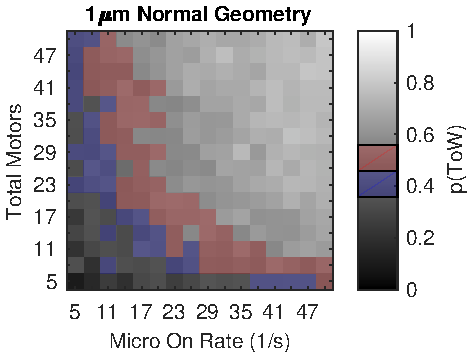
\includegraphics[width=7.75cm]{appendix1/n1000ToW.pdf}
\hspace{.5cm}
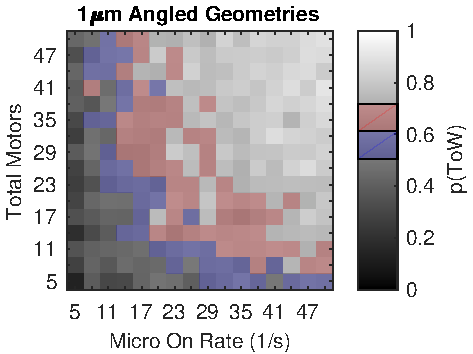
\includegraphics[width=7.75cm]{appendix1/angled1000ToW.pdf}
\\ \vspace{.5cm}
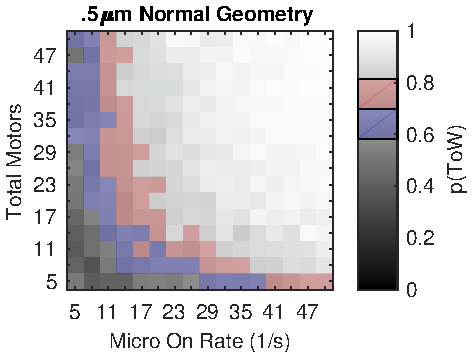
\includegraphics[width=7.75cm]{appendix1/n500ToW.pdf}
\hspace{.5cm}
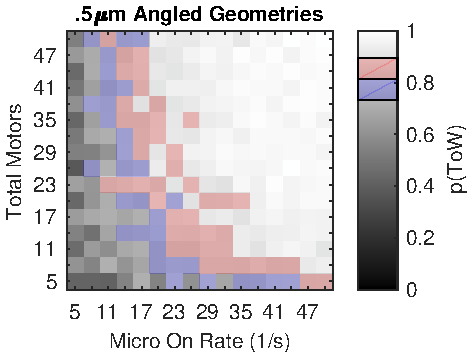
\includegraphics[width=7.75cm]{appendix1/angled500ToW.pdf}
\caption[ToW probabilities for varying combinations of the unknown parameters]{ToW probabilities for varying combinations of the unknown parameters\\
ToW probabilities are shown as grey scale heat maps for a range of parameter combinations. Those which yielded ToW probabilities within the experimental 95\% confidence interval are highlighted in color. Red highlighting indicates a probability above the experimental mean, blue highlighting below. All probabilities gathered from 300 cargos. For angled geometries, 150 acute runs were grouped with 150 obtuse runs.}
\label{fig:ToW_fit}
\end{figure}

%------------------------------------------------------------------------------------------------------------------------------
\subsubsection*{Robust transport constraint}

Experimental cargos are often observed to travel along the entire length of microtubules (\SI{10}{\micro\meter} or greater). Because single motor off rates are constrained by single molecule run length experiments \cite{Block1990,Milic2014,Li2016}, we can constrain acceptable combinations of motor number and on rate by looking at simulated cargo run length. An ensemble of cargos were simulated without the crossing MT and allowed to walk until either all motors detached from the MT or a motor head passed a point \SI{10}{\micro\meter} from where the cargo started. Results are shown in figure \ref{fig:run_length_fit}. In experiments, roughly half of cargos were observed to travel the entire length of the MT.

\begin{figure}
\centering
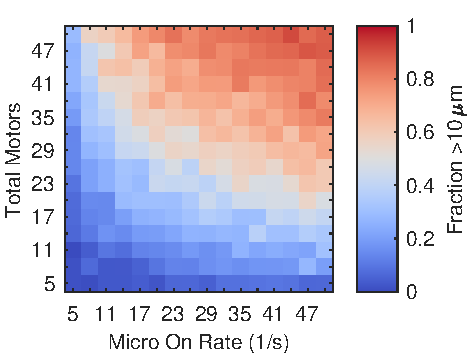
\includegraphics[width=7.75cm]{appendix1/10micronHeatmap.pdf}
\hspace{.5cm}
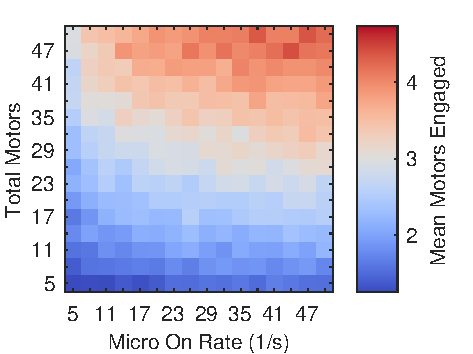
\includegraphics[width=7.75cm]{appendix1/n_ss}
\caption[Experimental observations inform selection of unknown parameters]{Experimental observations inform selection of unknown parameters \\
\textit{Left}: Fraction of cargos that travelled more than 10 microns are shown as a heat map for a range of parameter combinations. Fractions determined by simulation of 300 cargos. \\
\textit{Right}: Mean number of motors engaged on the MT at steady state is shown as a heat map for a range of parameter combinations. Values represent mean over 200 cargos. The number of motors engaged was assessed \SI{1.5}{\second} after the run began for each cargo. This time was long enough for cargos of all parameter combinations to reach steady state.}
\label{fig:run_length_fit}
\end{figure}

%------------------------------------------------------------------------------------------------------------------------------
\subsubsection*{Force constraint}

In experiments, force production of cargos was limited by the strength of the optical traps securing the bead handles. If generated forces were large enough, the forward bead handle was pulled out of its optical trap. Data for these cargos was discarded. The maximum force the bead handles could withstand was about \SI{7}{\pico\newton}, greater than the single motor stall force but less than the maximal stall force of two motors\added[id=MB,remark={Should cite the supplemental figure on this}]{}. Because experimental cargos often do not stall and geometric effects tend to keep all motors from exerting their maximal force on the bead handle at once, we expect there to be 2-3 motors exerting force on the bead handle.

Because simulated MTs are not dynamic, average or maximal simulated forces do not necessarily correspond to those one would expect to see experimentally. Therefore we investigate the number of motors simultaneously engaged on the MT at steady state, which estimates an upper limit for the number of motors simultaneously producing force.

To find the number of motors engaged on the MT, we simulate cargos walking along the primary MT without interference from a crossing MT. First, we simulate an ensemble of cargos and examine the average number of motors engaged over the ensemble as time progresses. After an initial transient, there is a period of time where neither the number of engaged motors nor the standard deviation thereof changes much. We call the average number of engaged motors during this time the steady state number. A survey of parameter combinations revealed that \SI{1.5}{\second} was long enough for cargos to come to steady state. Then, we check the average number of engaged motors at steady state for many parameter combinations. The results are shown in figure \ref{fig:run_length_fit}.

%------------------------------------------------------------------------------------------------------------------------------
\subsubsection*{Parameter selection}


A survey of figures \ref{fig:ToW_fit} and \ref{fig:run_length_fit} reveals that only parameter combinations with high numbers of total motors and low on rate fit the ToW probability and also match estimated run length and number of engaged motors. A manual search of parameter combinations in this region yielded $N=30$, $\kon^\text{micro}=\SI{10}{\per\second}$ as the best fit.

%%%%%%%%%%%%%%%%%%%%%%%%%%%%%%%%%%%%%%%%%%%%%%%%%
\section{Model Results} \label{sec:results}

Cargo trajectories were simulated forward in time as described in sections \ref{description} and \ref{sec:simulation}. Simulations were performed using the parameter values listed in table \ref{tab:params}. All parameter values used except microscopic on rate and total number of motors on the cargo are established in the literature or set by the experiment. Section \ref{param_fit} details how values for the unknown parameters were fit.

An ensemble of trajectories was simulated for a given geometry. Trajectories were categorized as described below, and probabilities of ToW and switching were derived. As shown in figure \ref{fig:trajectories}, the general behavior of simulated cargos was the same as experimental ones.

%**************************************************************************************************************
\subsection{Categorization of trajectories} \label{sec:rules}

Simulated trajectories were categorized using rules intended to emulate experimentally observed markers. Simulations began with the cargo outside of the ToW zone (section \ref{sec:ToW} and figure \ref{fig:heuristic}) and ended one of three ways: by the cargo detaching from the MT, by the cargo leaving the ToW zone on the primary MT, or by the cargo leaving the ToW zone on the crossing MT. The latter two cases were categorized as passes and switches, respectively. If the cargo detached from the primary MT before going by the intersection point, the run was discarded. If the cargo passed the intersection on the primary MT, but detached before leaving the ToW zone, the run was counted as a pass. Similarly, if the cargo was walking on the crossing MT but detached before leaving the ToW zone, the run was counted as a switch. Experimental runs were categorized using the same criteria.

Simulated cargos were marked as undergoing ToW when motors were attached to both MTs simultaneously for more than \SI{.25}{\second}. This time was selected as the minimum time in which a ToW would be detectable experimentally, given the camera frame rate. ToW time was measured as the total time during which motors were attached to both MTs and average values during ToW were accumulated during this period.

\begin{figure}
\centering
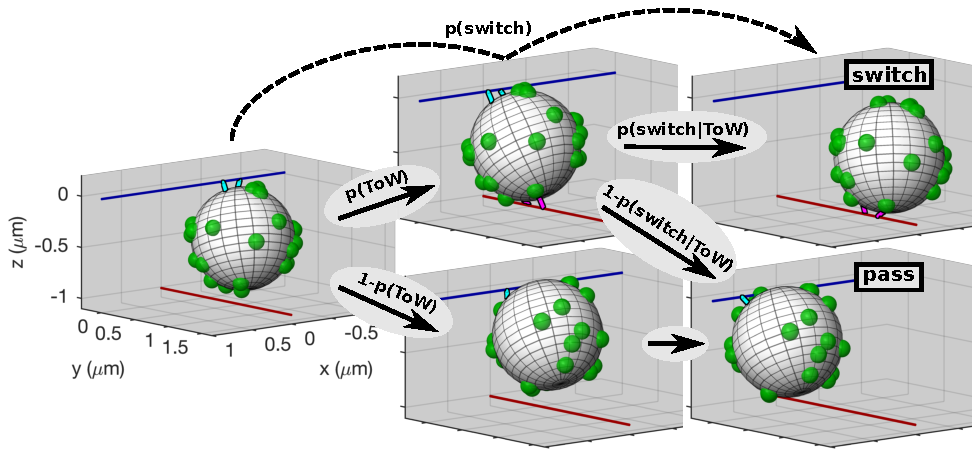
\includegraphics[width=6.5in]{appendix1/snapshots}
\caption[Snapshots from simulated cargo trajectories]{Snapshots from simulated cargo trajectories\\
During a simulation run, cargos begin outside the ToW zone with a single motor attached to the MT. Motors step stochastically, moving the cargo along the MT (\textit{left}). The cargo diffuses translationally as well as rotationally. When the cargo encounters the crossing MT, motors may bind and induce a ToW with $p(\text{ToW})$ (\textit{center,top}) or the cargo may go by the MT without any motors binding(\textit{center,bottom}). Cargos which do not ToW always pass. ToWs may end in the primary MT motor team becoming detached, resulting in a switch, with probability $p(\text{switch|ToW})$ (\textit{right,top}). Otherwise, the motor team on the crossing MT detaches, resulting in a pass (\textit{right,bottom}). To switch, a cargo must undergo ToW, then the crossing MT team must win the ToW. Therefore, the overall probability of switching $p(\text{switch})$ in given by $p(\text{ToW}) \times p(\text{switch|ToW})$.}
\label{fig:trajectories}
\end{figure}

%**************************************************************************************************************
\subsection{Encounter outcome dependance on MT geometry}

Ensembles of trajectories were simulated for varying separations and angles between the MTs. MT separations were varied from \SI{0}{\micro\meter} to \SI{1}{\micro\meter}, corresponding to 0 to 1 times the cargo diameter. Angles between the MTs were varied from nearly parallel to nearly anti-parallel. Figure \ref{fig:fractions} shows the resulting ToW and switch probabilities, along with the conditional probability of switching, given the cargo underwent ToW.

\begin{figure}
\centering
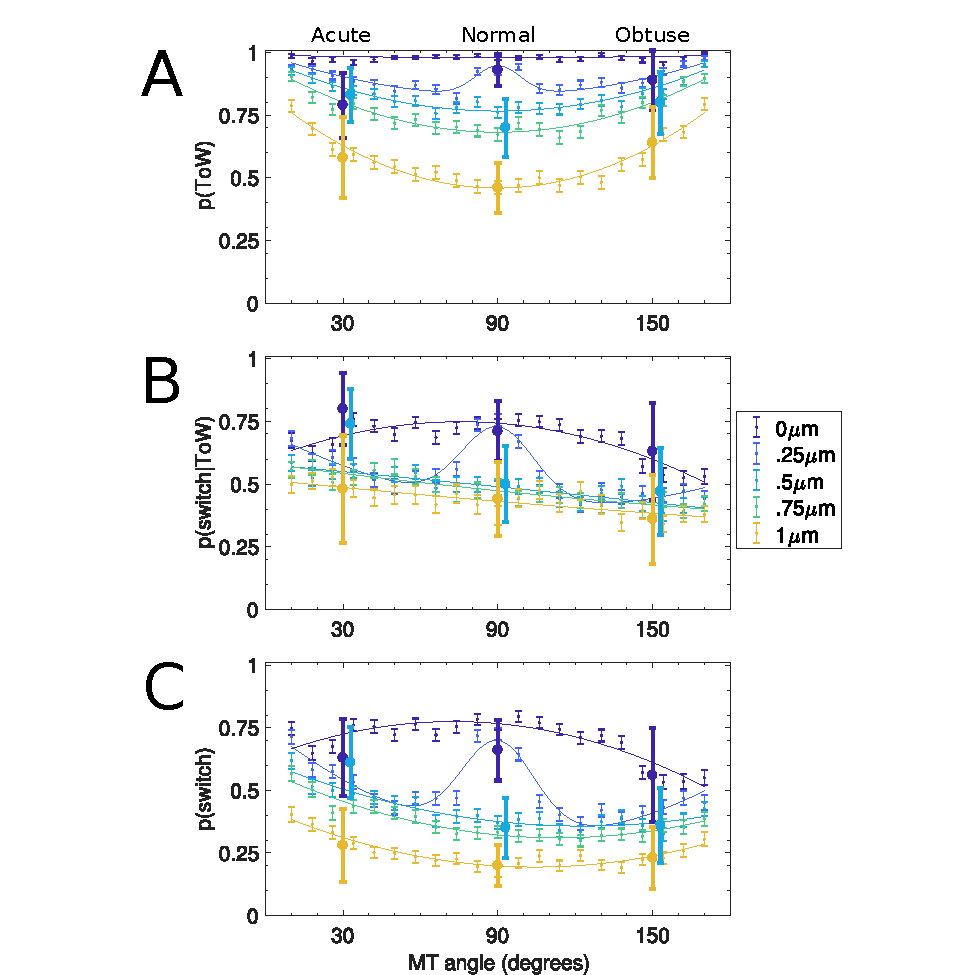
\includegraphics[width=6.5in]{appendix1/probs}
\caption[Probabilities of ToW and switching given ToW combine to explain switch probability]{Probabilities of ToW and switching given ToW combine to explain switch probability\\
\textit{A}: ToW probability as a function of the angle between the MTs is shown for separation distances corresponding to 0, 1/4, 1/2, 3/4 and 1 times the cargo diameter. Simulated data shown with thin bars representing standard error. Curves represent quadratic fits to simulated data for all but \SI{.25}{\micro\meter} separation distance, which is fit to a quadratic with an overlaid gaussian. Experimental data shown with think bars representing 95\% confidence interval.\\
\textit{B}: Conditional probability of switching, given the cargo undergoes ToW. Data represented as in \textit{A}.\\
\textit{C}: Overall switch probability. Data represented as in \textit{A}}
\label{fig:fractions}
\end{figure}

%**************************************************************************************************************
\subsection{Explanation of ToW probability} \label{sec:ToW}

In agreement with intuition, ToW probability increases with the distance the cargo must travel while able to reach both MTs simultaneously, which we call the ToW zone, denoted $x_\text{ToW}$. The extent of the ToW zone was calculated from geometry diagrammed in figure \ref{fig:heuristic}, and is given by
\begin{multline} \label{eq:ToW_zone}
x_\text{ToW}=2\frac{ \sqrt{4 (L+R+R_{MT})^2-\left( (\xmt^1-\xmt^2)\cdot \hat{z} \right)^2} }{\norm{\dmt^1 \cross \dmt^2}} \\
= 2\frac{ \sqrt{4 (L+R+R_{MT})^2-\left( \text{separation distance} \right)^2} }{\sin(\text{MT angle})}.
\end{multline}
The probability a cargo will undergo ToW can then be understood as a competition between the rate at which the cargo binds to the crossing MT, which happens at a rate which we denote $\kon^\text{macro}$, and the rate it leaves the ToW zone, which happens at a rate given by the cargo velocity (equal to the maximum single motor velocity $v$) divided by the ToW zone length. Thus,
\begin{equation} \label{eq:rate_war}
p(\text{ToW})=\frac{ \kon^\text{macro}}{\kon^\text{macro} +  \frac{v}{x_\text{ToW}}}.
\end{equation}
The rate at which the cargo attaches to the crossing MT, $\kon^\text{macro}$, is in general a complex function of geometry as well as motor and cargo parameters. However, for this heuristic analysis we assume it is constant across different geometries. If we fit the macro on rate to the experimental data on ToW probability, we recover the qualitative features of the full simulation result as shown in figure \ref{fig:heuristic}.

\begin{figure}
\centering
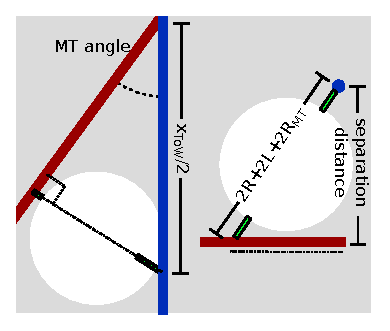
\includegraphics[width=6cm]{appendix1/ToWzone}
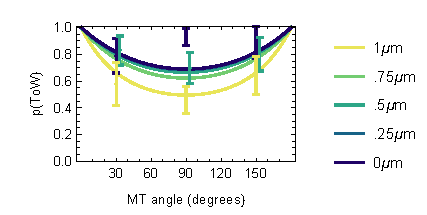
\includegraphics[width=10cm]{appendix1/heuristicSIM.pdf}
\caption[A heuristic model matches qualitative features of ToW probability]{A heuristic model matches qualitative features of ToW probability\\
\textit{Left}: Diagram of the ToW zone. The ToW zone is defined as the distance along the primary MT in which the cargo can reach the crossing MT. Its length was calculated geometrically and is given by equation \ref{eq:ToW_zone}. Primary MT is shown in blue, crossing MT in red, motors in green and cargo in white. \\
\textit{Right}: Solutions to the heuristic model for ToW probability. The heuristic model poses the probability of undergoing ToW as the the probability of the cargo binding (with constant binding rate) to the crossing MT before leaving the ToW zone and is given in equation \ref{eq:rate_war}. Experimental probabilities are shown with error bars representing 95\% confidence interval. Bars for data at \SI{.5}{\micro\meter} shifted slightly to aid the eye. Solutions plotted with $\kon^\text{macro}$ set to \SI{1}{\per\second}. 
}
\label{fig:heuristic}
\end{figure}

%------------------------------------------------------------------------------------------------------------------------------
\subsubsection*{Steric effects strongly influence ToW probabilities in \SI{0}{\micro\meter} and \SI{.25}{\micro\meter} geometries}

A comparison of figures \ref{fig:heuristic} and \ref{fig:fractions}A reveals that the heuristic model captures the features of ToW probability for MT separations \SI{.5}{\micro\meter} and greater very well. However, it fails to reproduce features of the simulated data at \SI{.25}{\micro\meter} and \SI{0}{\micro\meter}. This failure shows that the peak in ToW probability near the normal for \SI{.25}{\micro\meter} separation and the overall high ToW probability at \SI{0}{\micro\meter} must result from effects not considered in the heuristic model. As discussed in the main text, steric interactions play a large role.

%**************************************************************************************************************
\subsection{Explanation of conditional probability of switching given ToW}

The complex dependence of conditional probability of switching on geometry is not intuitive and warrants further investigation. To this end, we show the mean number of motors engaged on each MT during ToW, the mean forces exerted on the motor teams during ToW, the ToW time, and how each of these depends on the MT geometry in figure \ref{fig:ToW_forces}. Below we explain the behavior of the simulated conditional probability of switching on geometry using these results.

\begin{figure}
\centering
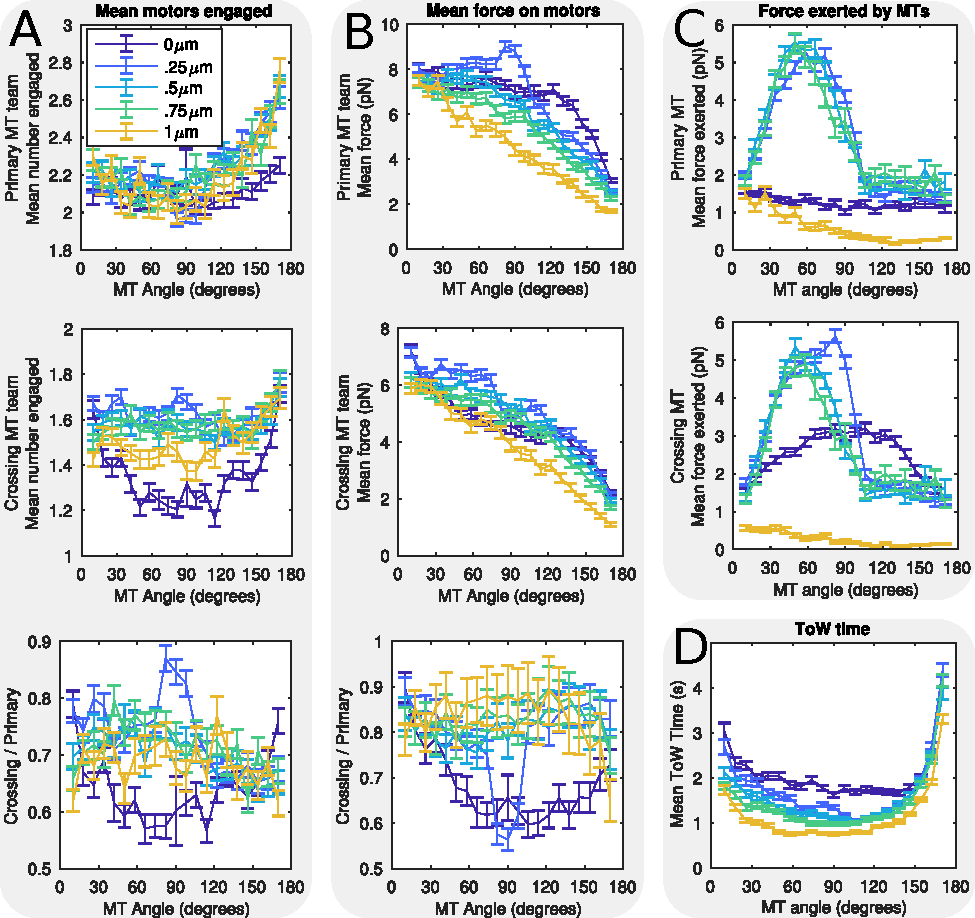
\includegraphics[width=6.5in]{appendix1/forces}
\caption[Numbers engaged, forces and ToW times explain conditional probability of switching]{Numbers engaged, forces and ToW times explain conditional probability of switching\\
\textit{A}: Mean number of motors engaged during ToW for primary and crossing MT teams. The numbers are shown as a function of MT angle. Below, the ratio of mean motors engaged on the crossing MT to the primary MT is shown. Separation distances are colored as described in the legend in the top panel of \textit{A}. Error bars represent standard error of the mean. \\
\textit{B}: Mean force experienced by the motor teams on the primary and crossing MTs during ToW. Forces are shown as a function of angle. Below, the ratio of the forces on the crossing MT team to the forces on the primary MT team is displayed. Data represented as in \textit{A}.\\
\textit{C}: Mean steric force exerted by the primary and crossing MTs during ToW. Forces shown as a function of angle and represented as in \textit{A}.
\textit{D}: Mean ToW time as a function of angle between the MTs. ToW time is the total time motors are engaged on both MTs. Data represented as in \textit{A}.}
\label{fig:ToW_forces}
\end{figure}

%------------------------------------------------------------------------------------------------------------------------------
\subsubsection*{\SI{1}{\micro\meter} near-normal geometries}

At \SI{1}{\micro\meter} separation distance, the cargo can not sterically interact with both MTs at once. Since forces exerted by the MTs are minimal (figure \ref{fig:ToW_forces}C), motor teams in these ToWs pull directly on each other, as evidenced by high forces on the motor teams and a ratio near 1, shown in figure \ref{fig:ToW_forces}B. Furthermore, ToW times are short (figure \ref{fig:ToW_forces}D), meaning the crossing MT team often only gets one chance to cause a switch. One might expect, then, that since the ratio of crossing MT to primary MT motor number is $\approx .7$ (figure \ref{fig:ToW_forces}A), switches would happen about 30\% of the time. However, a ToW between motor teams of different numbers is not directly determined by motor numbers. The slow increase of unbinding rate above stall gives the smaller team a significant chance to win the ToW, leading to an overall probability of switching higher than 30\%, but still below 50\%.

%------------------------------------------------------------------------------------------------------------------------------
\subsubsection*{\SI{1}{\micro\meter} acute geometries}

Conditional probabilities of switching at \SI{1}{\micro\meter} are slightly higher for acute geometries  than they are near the normal. As in the latter, motors pull directly on each other during ToWs, evidenced by high forces in figure \ref{fig:ToW_forces}B. However, an asymmetry exists between a ToW won by the crossing MT motor team and the primary MT motor team in acute geometries. When the primary MT motor team wins a ToW, the cargo continues on through the ToW zone (which is longer for more acute geometries, see equation \ref{eq:ToW_zone}). During this time motors may again bind to the crossing MT, giving another chance for a switch. Evidence of this effect can be seen in the longer ToW times shown in figure \ref{fig:ToW_forces}D. However, when the crossing MT team wins a ToW, the cargo is likely to diffuse down and away from the primary MT and avoid rebinding. This effect drives switching up slightly for acute geometries compared to near-normal.

%------------------------------------------------------------------------------------------------------------------------------
\subsubsection*{\SI{1}{\micro\meter} obtuse}

Unlike in near-normal and acute geometries at \SI{1}{\micro\meter}, motors in obtuse geometries feel low average forces, as shown in figure \ref{fig:ToW_forces}B. ToW times are long, as seen in figure \ref{fig:ToW_forces}D, because MT alignment is close to parallel and motors walk in nearly the same direction. Motors do not feel significant load until the cargo has moved far enough from the intersection that the distance from MT to MT is greater than twice the bead diameter. These long periods of walking under low force turn the ToW into a competition of processivity as much as force. While a smaller motor team can compete against a larger motor team in a force competition, processivity grows quickly with motor number, so larger motor teams are more likely to win a processivity competition. Because there are on average more motors on the primary MT team, the probability of switching goes down as the distance walked goes up with more obtuse angles.

%------------------------------------------------------------------------------------------------------------------------------
\subsubsection*{\SI{.5}{\micro\meter} near-normal geometries}

In \SI{.5}{\micro\meter} geometries, the cargo must hurdle up and over the crossing MT to pass. If the cargo is underneath the primary MT, the primary MT motors are loaded as they pull the cargo into the crossing MT, but the cargo cannot pass the intersection until it is out from underneath the primary MT. In near-normal geometries, the crossing MT team assists this process by pulling the cargo out toward the plus end of the crossing MT. While this is taking place, the primary MT motors continue to be loaded. This load sometimes causes primary MT motors to unbind, leading to a weaker team on average. As crossing MT motors walk, the force from the primary MT motors is shifted from the crossing MT to the crossing MT motor team. In the end, this interaction has similar dynamics to the ones described in the \SI{1}{\micro\meter} near-normal geometries, albeit with a primary MT motor team that is now weaker on average. This slightly biases the ToW toward the crossing MT team relative to \SI{1}{\micro\meter} near-normal geometries, resulting in a ToW probability near 50\%.

%------------------------------------------------------------------------------------------------------------------------------
\subsubsection*{\SI{.5}{\micro\meter} acute geometries}

Unlike in near-normal geometries at \SI{.5}{\micro\meter}, the crossing MT motors do not aid hurdling behavior in acute geometries. In fact, they impede hurdling; when the crossing MT motors engage, they act to wedge the cargo between the MTs, described as "chop-sticking" in the main text. This effect can be seen in the high forces exerted by the MTs at these geometries shown in figure \ref{fig:ToW_forces}C. Because crossing MT motors impede hurdling and the cargo must travel beyond the intersection to pass, crossing MT motors often get multiple chances to cause a switch, indicated by long ToW times in figure \ref{fig:ToW_forces}D. This leads to the conditional probability of switching rising 50\%.

%------------------------------------------------------------------------------------------------------------------------------
\subsubsection*{\SI{.5}{\micro\meter} obtuse geometries}

As in \SI{.5}{\micro\meter} near-normal geometries, crossing MT motors aid hurdling in \SI{.5}{\micro\meter} obtuse geometries. Additionally, like obtuse geometries at \SI{1}{\micro\meter} separation distance, ToW times are long (figure \ref{fig:ToW_forces}D) and forces are low (figure \ref{fig:ToW_forces}B). As described, this biases the ToW toward the larger motor team on the primary MT and results in less switching.

%------------------------------------------------------------------------------------------------------------------------------
\subsubsection*{\SI{.25}{\micro\meter} and \SI{.75}{\micro\meter} geometries}

The conditional probability of switching in \SI{.25}{\micro\meter} and \SI{.75}{\micro\meter} geometries is similar to that of \SI{.5}{\micro\meter} geometries, indicating the same mechanisms are at play. There is a significant deviation at angles near the normal in \SI{.25}{\micro\meter} geometries. At these angles, the crossing MT becomes a very effective barrier to progress of the cargo. Because the crossing MT is above the cargo equator, steric forces from the crossing MT tend to push the cargo back down, causing it to get stuck below the intersection. This effect can be seen in the high MT forces near normal in figure \ref{fig:ToW_forces}C. Stuck cargos are more likely to switch, leading to an overall high switching probability.

%------------------------------------------------------------------------------------------------------------------------------
\subsubsection*{\SI{0}{\micro\meter} near-normal geometries}

As explained in the main text, cargos may only pass two ways in \SI{0}{\micro\meter} geometries: by the cargo hurdling up and over the crossing MT, or by monkey-barring. Since cargos experience a gravitational force, they are likely to encounter the intersection below the crossing MT and not be able to hurdle. Because successful monkey-barring is a process which requires two rare events, this leads to a high probability of switching.

%------------------------------------------------------------------------------------------------------------------------------
\subsubsection*{\SI{0}{\micro\meter} acute geometries}

Because the ToW zone is longer in acute geometries than near-normal, cargos are more likely to undergo several ToW events. This is reflected in the long ToW times at acute geometries shown in figure \ref{fig:ToW_forces}D. In the opposite effect of that in \SI{.5}{\micro\meter} geometries, these longer ToWs lead to less switching in \SI{0}{\micro\meter} geometries. This is because these longer ToWs give the cargo more chances to monkey-bar and pass the intersection.

%------------------------------------------------------------------------------------------------------------------------------
\subsubsection*{\SI{0}{\micro\meter} obtuse geometries}

Conditional probability of switching falls as angles become closer to parallel for \SI{0}{\micro\meter} separation distance, and approaches 50\%. The forces on the cargo in these geometries are such that motors on the crossing MT tend to pull the cargo up and over the top of the intersection. This leads to greater ease of passing because the crossing MT no longer blocks progress of the primary MT motor team when the cargo is above the plane.

%\newpage
%
%\vspace*{2\baselineskip}
%\centerline{\textbf{\LARGE Captions for supplemental movies}}
%\vspace{4\baselineskip}
%
%\begin{itemize}[label={}]
%
%\item \textbf{Supplement Movie 1.} Intersection geometry: \SI{0.5}{\micro\meter} separation, \ang{90} angle.  MC engages in ToW, and ultimately passes. For detailed analysis of this event, see Fig. 2A,B,D. The video has been rescaled 3X for clarity.
%
%\item \textbf{Supplement Movie 2.} Intersection geometry: \SI{0.5}{\micro\meter} separation, \ang{90} angle.  MC engages in ToW, and ultimately switches. For detailed analysis of this event, see Fig. 2C. The video has been rescaled 3X for clarity.
%
%\item \textbf{Supplement Movie 3.} Intersection geometry: \SI{1}{\micro\meter} separation, \ang{90} angle.  MC engages in ToW, and ultimately switches.
%
%\item \textbf{Supplement Movie 4.} Intersection geometry: \SI{1}{\micro\meter} separation, \ang{90} angle.  MC engages in ToW and ultimately passes.
%
%\item \textbf{Supplement Movie 5.} Intersection geometry: \SI{0.5}{\micro\meter} separation, \ang{90} angle.  MC engages in ToW, "hurdles" over the crossing MT, and ultimately switches.  
%
%\item \textbf{Supplement Movie 6.} Intersection geometry: \SI{0.5}{\micro\meter} separation, \ang{90} angle.  MC engages in ToW, "hurdles" over the crossing MT, and ultimately passes. 
%
%\item \textbf{Supplement Movie 7.} Intersection geometry: \SI{0}{\micro\meter} separation, \ang{90} angle. The motors engaged on the primary MT are initially blocked. Other motors then engage the crossing MT, and the MC switches.
%
%\item \textbf{Supplement Movie 8.} Intersection geometry: \SI{0}{\micro\meter} separation, \ang{90} angle. MC ToWs and then and ultimately passes via "monkey-barring."
%
%\item \textbf{Supplement Movie 9.} Intersection geometry: \SI{0}{\micro\meter} separation, \ang{90} angle. Simulated viscosity: \SI{1}{\pascal\second} (1000x as viscous as water).  MC ToWs and then and ultimately switches.
%
%\item \textbf{Supplement Movie 10.} Intersection geometry: \SI{0.5}{\micro\meter} separation, acute angle. When the MC engages in a ToW, the ability to hurdle is suppressed ("chop-sticking").  The MC ultimately switches.  
%
%\end{itemize}
%
%\newpage
%
%\newrefcontext[labelprefix=S]
%\printbibliography
%
%\end{document}


\end{document}
